\hypersetup{linkcolor=blue, citecolor=red}

\chapter{Metodi di Gestione e Manutenzione per Reti Sicure} \label{chap:3}

La sola implementazione delle soluzioni descritte precedentemente per costruire una rete sicura non basta. È fondamentale adottare una metodologia per la gestione e la manutenzione delle reti, al fine di preservare l'integrità e la sicurezza nel tempo.
Vedremo i processi e le best practice per una corretta amministrazione delle infrastrutture di rete. Particolare attenzione sarà dedicata alla definizione di procedure standardizzate che permettano di mantenere nel tempo un elevato livello di sicurezza, riducendo al minimo gli errori umani e le vulnerabilità derivanti da configurazioni inappropriate.\\
L'obiettivo è quello di identificare un framework operativo che consenta agli amministratori di rete di gestire in modo efficace e sistematico le complesse infrastrutture moderne, bilanciando le esigenze di sicurezza con quelle di performance e disponibilità del sistema.

%\newpage

\section{Framework e Politiche di Sicurezza}
Per una gestione efficace bisogna costruire delle linee guida e seguire degli standard all'interno dell'azienda. Analizziamo alcuni dei framework più conosciuti.
    \subsection{ISO/IEC 27001}
    L'Organizzazione Internazionale per la Normazione è la più importante organizzazione a livello mondiale per la definizione di norme tecniche che, insieme alla Commissione Elettrotecnica Internazionale, hanno redatto un documento per definire dei requisiti specifici per l'implementazione di un Sistema di Gestione della Sicurezza delle Informazioni (SGSI). Questo documento è fondamentale per aiutare le aziende a mantenere la sicurezza delle loro informazioni. 
    Data la costante crescita delle tecnologie, questo standard viene aggiornato periodicamente, con l'ultima versione redatta nel 2022. Lo scopo di questo standard è certificativo, permettendo di costituire un sistema completo per garantire la gestione della sicurezza nella tecnologia dell'informazione. \\
     La norma  si basa sul modello PDCA (Plan-Do-Check-Act) e segue un approccio basato sulla gestione del rischio. I punti principali di questo approccio sono:
     
     \begin{itemize}
        \item Pianificazione e Progettazione. In particolare, qua è richiesta una fase di risk assessment, che viene suddivisa in:
        \begin{itemize}
            \item Identificazione dei rischi.
            \item Analisi e valutazione.
            \item Selezione degli obiettivi di controllo e attività di controllo per la gestione dei rischi.
            \item Assunzione del rischio residuo da parte del management.
            \item Definizione dello Statement of Applicability, ossia gli obiettivi di controllo adottati e i controlli implementati dall'organizzazione rispetto ad una lista di obiettivi di controllo previsti dalla norma. 
        \end{itemize}
        \item Implementazione (processi operativi).
        \item Monitoraggio.
        \item Miglioramento.
     \end{itemize}
     
    Di fondamentale importanza è l'Annex A “Control objectives and controls” che contiene i 133 “controlli” a cui l'organizzazione che intende applicare la norma deve attenersi; infatti, questo allegato descrive le azioni necessarie per garantire la sicurezza dei sistemi IT. Si occupa anche di importanti aspetti della sicurezza dei dati, come la sicurezza fisica, la protezione legale, la gestione delle risorse umane e le questioni organizzative.
         
     Questa norma è applicabile a tutte le imprese o aziende pubbliche, dato che non si basa su uno specifico settore di business o organizzazione. Bisogna tener presente che l'adozione e gestione di un SGSI richiede un impegno di risorse significativo e quindi deve essere seguita da un ufficio specifico.
     
        \subsubsection{ISO/IEC 27002}
        Questo è un documento aggiuntivo costituito da una raccolta di “best practices” che possono essere adottate per soddisfare i requisiti della norma ISO 27001 al fine di proteggere le risorse informative. A differenza della norma 27001, la 27002 non è certificabile in quanto è una raccolta di semplici raccomandazioni. Anche questo documento, seppur non certificabile, ha la sua importanza tecnica proprio per le linee guida che fornisce ed è complementare alla 27001, andando a spiegare ogni controllo presentato nell'allegato A prima citato e come essi possano essere implementati.

\newpage

    \subsection{NIST Cybersecurity Framework - CSF}
        Sviluppato dal National Institute of Standards and Technology, NIST\footnote{Fonte: NIST (\url{https://www.nist.gov/}) }, il Cybersecurity Framework è un insieme di linee guida  progettate per aiutare le organizzazioni a valutare e migliorare la loro capacità di prevenire, rilevare e rispondere ai rischi di sicurezza informatica. È stato progettato per essere flessibile e adattabile, fornendo una guida di alto livello che consente alle singole organizzazioni di determinare le specifiche di implementazione in base alle loro esigenze uniche e ai profili di rischio. Sebbene ampiamente elogiato, è stato criticato per i costi e la complessità connessi alla sua attuazione, in particolare per le piccole e medie imprese. 
        Il CSF è formato da 3 componenti principali:
        \begin{itemize}
            \item Core. Il quale offre un insieme strutturato di attività e linee guida correlate ai diversi aspetti della cybersecurity. Al suo interno, definisce 6 funzioni fondamentali, articolate in 23 sottocategorie distinte, tra cui:
                \begin{itemize}
                    \item \textbf{Identificare}. Questa funzione è orientata a rafforzare la consapevolezza sugli asset aziendali e sui rischi correlati, ottimizzando anche i processi di gestione patrimoniale.
                    \item \textbf{Proteggere}. La finalità di questa funzione è preservare l'integrità di dati sensibili e infrastrutture tecnologiche, rilevando accessi illeciti, violazioni e potenziali attacchi informatici.
                    \item \textbf{Rilevare}. Questa funzione include una sorveglianza sistematica degli incidenti di cybersecurity, attraverso attività come l'identificazione di intrusioni e il tracciamento log e il monitoraggio degli eventi.
                    \item \textbf{Rispondere}. Lo scopo di questa funzione è di attivare tempestive contromisure in caso di incidenti, attraverso una gestione coordinata delle risorse al fine di contenere gli impatti e accelerare il ripristino delle funzionalità.
                    \item \textbf{Recuperare}. Si focalizzata sul ripristino dell'operatività post-incidente, questa funzione garantisce una transizione efficiente verso la regolare attività, integrando al contempo azioni correttive per potenziare le difese future.
                    \item \textbf{Govern}. Introdotta con l'aggiornamento 2024 del framework, questa funzione rappresenta un nuovo pilastro strategico: guida all'integrazione coerente delle altre cinque funzioni, estendendo la sua applicabilità a tutti gli asset tecnologici dell'organizzazione.

                    
                \end{itemize}
        \begin{samepage}
            \item Implementation Tiers. Si tratta di livelli progettati per supportare le organizzazioni nella valutazione dell'efficacia delle proprie strategie di cybersecurity e del loro grado di evoluzione. La suddivisione prevede 4 livelli, così definiti:
            \begin{itemize}
                \item \textbf{Tier 1 – Parziale}.
                    Le organizzazioni dimostrano una consapevolezza parziale delle minacce informatiche, gestendo la sicurezza con criteri disorganizzati e privi di un piano strutturato.
                \item \textbf{Tier 2 – Informato}.
                    Le organizzazioni delineano una strategia di gestione del rischio più articolata, avviando l'integrazione graduale di un programma cybersecurity strutturato e documentato.
                \item \textbf{Tier 3 – Ripetibile}.
                    Le organizzazioni dispongono di un framework cybersecurity consolidato, accompagnato da meccanismi di mitigazione del rischio e un monitoraggio periodico delle prestazioni di sicurezza.
                \item \textbf{Tier 4 – Adattivo}.
                    Le organizzazioni adottano un approccio alla cybersecurity avanzato e dinamico, caratterizzato da un orientamento proattivo alla gestione del rischio, ai processi di ottimizzazione continui e alla capacità di risposta rapida ed efficace agli incidenti.

            \end{itemize}
        \end{samepage}
            \item Profiles. Strumenti flessibili che permettono di personalizzare il framework in base alle esigenze organizzative e al profilo di rischio. Tipicamente, le organizzazioni definiscono un “Profilo corrente” per catalogare le pratiche e i risultati già attivi in ambito sicurezza. In seguito, costruiscono un “Profilo obiettivo” per identificare i traguardi desiderati e pianificare le iniziative di transizione. Alternativamente, è possibile adottare un profilo predefinito, calibrato su standard di settore o su specificità operative rilevanti.
        \end{itemize}
        
        Anche questo framework ha subito diversi aggiornamenti per stare al passo con la tecnologia, arrivando all'ultima versione, la 2.0 del 2024, aggiungendo nuove linee guida sulla governance della sicurezza informatica.

        \subsubsection{Unione tra ISO/IEC 27001 e NIST CSF}
        L'unione tra i due framework rappresenta un approccio strategico vincente per rinforzare la sicurezza informatica di un'organizzazione, permette di potenziare la capacità di gestione del rischio, di ottenere una certificazione internazionale e di promuovere un miglioramento continuo alle pratiche di sicurezza, ma nonostante i vantaggi, l'integrazione presenta sfide significative.
        Mantenere infatti l'allineamento dei diversi requisiti, così come la certificazione nel caso di ISO 27001, personalizzando allo stesso tempo gli approcci per adattarli al proprio contesto, come suggerito dal CSF, non è un lavoro da poco.
        Le organizzazioni devono gestire queste difficoltà con attenzione per definire una strategia di cybersecurity coerente, in grado di affrontare sia le minacce in evoluzione sia le richieste normative, garantendo al contempo una solida gestione della sicurezza delle informazioni.
        
        Per affrontare queste sfide, sviluppare un piano di integrazione che combini i punti di forza di entrambi i modelli e che implementi i controlli, dando priorità ad aree critiche necessarie, è fondamentale per far convivere entrambi i framework insieme creando una struttura solida.
        Le organizzazioni disposte a investire in un programma completo di sicurezza informatica che incorpora entrambi i modelli possono trovare vantaggi strategici a lungo termine. Stabilendo una solida base con ISO 27001 e migliorando la flessibilità attraverso CSF, le organizzazioni possono sviluppare una strategia di sicurezza informatica solida e resiliente su misura per le loro esigenze e obiettivi unici \cite{linkedin_iso_csf}, \cite{Comparison_CSF_ISO}.

        \subsection{COBIT 2019}
            Tra i vari framework troviamo anche il COBIT, ossia il Control Objectives for Information and Related Technologies, sviluppato in particolare per la governance IT, che garantisce sicurezza, integrità e conformità normativa adattandosi bene a organizzazioni di ogni tipo, grandi o piccole.
            La sua struttura è composta da 6 punti chiave, ed essi sono:
            \begin{itemize}
                \item \textbf{Processi}. Attività e pratiche necessarie per raggiungere specifici obiettivi IT.
                \item \textbf{Strutture Organizzative}. Organi che prendono decisioni nella governance.
                \item \textbf{Principi, politiche e framework}. Linee guida per allineare l'IT alla società.
                \item \textbf{Flussi di informazioni}. Dati essenziali per la governance.
                \item \textbf{Cultura, etica e comportamenti}. Come i comportamenti di un individuo o di un gruppo impattano sulla governance.
                \item \textbf{Persone, skill e competenze}. Risorse umane critiche per raggiungere gli obiettivi di governance.
            \end{itemize}
            L'approccio strutturale di questo modello è molto flessibile e permette alle organizzazioni di adattarsi al framework in base alle loro necessità e lo rende facile da implementare. Questo modello promuove anche il cambiamento, aiutando le aziende ad adattarsi agilmente ai cambiamenti tecnologici; inoltre facilita la comunicazione e la collaborazione tra i diversi software interni di un business, supportando il management IT \cite{cobit_overview}.
            Questo modello è sicuramente il più adatto per la manutenzione continua e il management di una rete, essendo stato pensato per questo, fornendo allo stesso tempo solidi principi di sicurezza. Fornisce una struttura e un metodo d'approccio chiaro che cerca di legarsi agli obiettivi aziendali \cite{analysis_cobit_csf_iso27001}. Si concentra molto sull'importanza della manutenzione, sul controllo della rete, cercando sempre una risposta proattiva alla sicurezza, tenendo conto anche del fattore umano. Allo stesso tempo, la troppa flessibilità di questo framework e i diversi controlli che ha possono essere travolgenti per una società con poche risorse, in particolare quelle che non hanno un reparto IT dedicato \cite{cobit_fortinet_strengths_weaknesses}.

        \subsection{Politiche e Strutture Interne}
            La chiara definizione dei ruoli e delle responsabilità è un pilastro fondamentale per creare una governance efficace della sicurezza informatica. Senza una struttura organizzativa ben delineata, anche le policy più rigorose rischiano di rimanere teoriche. Vediamo l'importanza di alcuni ruoli come il Chief Information Security Officer, CISO, il responsabile strategico della sicurezza informatica il quale ha un ruolo trasversale che collega la direzione esecutiva, i reparti operativi e gli standard normativi. Questa figura si occupa infatti di sviluppare e implementare processi e sistemi sicuri per prevenire, rilevare e recuperare da attacchi, di definire gli obiettivi a lungo termine, di allineare il rischio aziendale ai vari framework di cui abbiamo parlato in precedenza e di implementare le policy di sicurezza che l'azienda deve seguire. Si occupa inoltre di allocare fondi per gli strumenti tecnologici, per la formazione del personale e di progettare e realizzare il piano di cybersecurity aziendale, per tenere al sicuro le risorse informatiche societarie.
            Si assume la responsabilità di garantire l'aderenza a normative come il GDPR (normativa per la privacy\footnote{Fonte: Wikepedia (\url{https://it.wikipedia.org/wiki/Regolamento_generale_sulla_protezione_dei_dati})}) e altre. Il suo ruolo è estremamente versatile, con compiti che non si limitano alla sicurezza informatica ma anche alla gestione aziendale, per cui non bastano solide basi in ambito IT ma sono necessarie anche competenze in ambito finanziario e amministrativo~\cite{ciso_cisco}. Questo ruolo in genere nelle imprese di medio-piccole dimensioni viene ricoperto da un membro del personale IT se presente, altre volte viene appaltato esternamente, mentre nel 40\% dei casi viene completamente ignorato \cite{ciso_csm_and_percentage}. Non in tutte le grandi imprese invece viene definito questo ruolo, infatti spesso viene affidato al CIO, Chief Information Officer, il quale si occupa però di tutta l'area IT e non solo della sicurezza; questo può portare a una negligenza di quest'ultima.
            Con il passare del tempo, la figura del CISO si è sempre più affermata e insieme a questa si è andato ad affiancare il ruolo di Cyber Security Manager. Questa figura ha un ruolo più tecnico ma meno manageriale rispetto al CISO, con il quale divide la responsabilità della sicurezza informatica aziendale. Contribuisce alla stesura delle policy di sicurezza e si occupa di farle rispettare, valuta rischi minacce e possibili conseguenze e gestisce il piano di Incident Response \cite{ciso_csm_and_percentage}.


\section{Monitoraggio della Rete}
    Il monitoraggio della rete è un aspetto fondamentale non solo per il corretto funzionamento o per il controllo delle performance di queste, ma anche per la loro sicurezza. Queste tecnologie si occupano di identificare componenti del sistema lenti e/o compromessi, così da poter rilevare, rispondere e mitigare potenziali attacchi per garantire la sicurezza del sistema. Al giorno d'oggi sono diverse le soluzioni per monitorare il network, come l'analisi del traffico, l'alerting in tempo reale e altre.
    Analizziamo ora i diversi tipi di monitoraggio del traffico.

    
    \subsection{Active Network Monitoring}
        Consiste nel generare traffico con pacchetti specifici all'interno della rete per testare la performance, l'availability e la reattività di quest'ultima. Questa tecnica di monitoring ha un approccio proattivo che permette la simulazione di breach nella rete per vedere la risposta del network sotto varie condizioni, misurando la performance con metriche tipo il response time, la latency, la percentuale di pacchetti persi e il throughput. Questa soluzione coinvolge l'implementazione di monitoring agents o sensori in punti strategici della rete per monitorare il traffico end-to-end che permettono il funzionamento prima descritto. Questo tipo di monitoraggio è comodo per una rete grande in quanto è scalabile e accomoda anche sistemi distribuiti \cite{paper_net_monitoring}.

        Anche se alcune grandi aziende potrebbero sviluppare dei propri tool di monitoring in-house, alcune imprese potrebbero preferire la possibilità di fare out-sourcing di questo servizio. Tra gli applicativi leader per le grandi imprese abbiamo SolarWinds\footnote{\label{solarwinds_site} Sito: (\url{https://www.solarwinds.com/})}, dato che è in grado di gestire reti complesse grazie alla sua scalabilità. Questo strumento è in grado di offrire rapporti dettagliati della rete, real-time monitoring, alerts automatici e altro. Questo applicativo comporta una spesa iniziale non solo per il programma in sé quanto per la difficoltà di gestione \cite{paper_net_monitoring}.

        \begin{figure}[H]
            \centering
            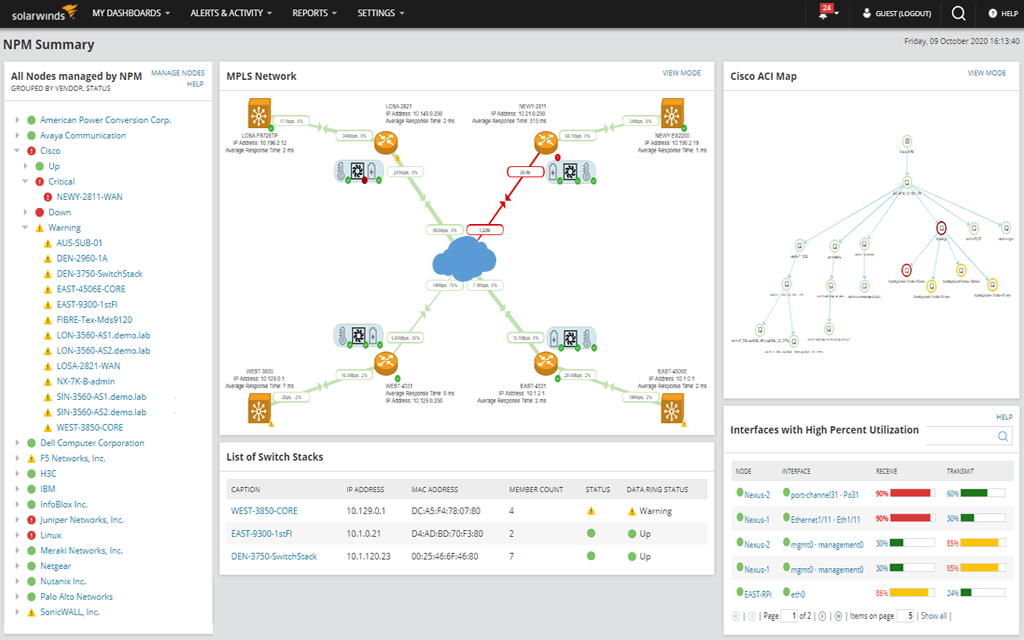
\includegraphics[width=1.0\textwidth]{Immagini/solar_wind_dashboard.png}
            \caption{Pannello di controllo SolarWinds\footref{solarwinds_site}.}
            \label{fig:solarwinds_dashboard}
        \end{figure}

    \subsection{Passive Network Monitoring}
        Questo tipo di monitoring cattura il traffico della rete implementando sensori al suo interno. A differenza dell'Active Monitoring, questo metodo non è proattivo, non interferirà quindi con le operazioni della rete, ma osserva semplicemente il traffico, fornendo un'analisi in tempo reale anche sui dati passati, facilitando l'identificazione di un pattern. Questi strumenti sono utili per individuare la causa di anomalie della rete, misurare la performance delle applicazioni, analizzare il comportamento della rete, anche durante attacchi esterni, mantenendo dei log dettagliati dell'attività nel network. Nelle varie implementazioni di questo tool non è raro trovare dei strumenti di monitoring chiamati “network tap” che catturano i pacchetti, analizzandone il contenuto ed estraendone informazioni importanti sulla performance, sicurezza e comportamento del network \cite{obkio_net_monitors}.

        Questo tipo di monitoraggio viene preferito quando si vogliono catturare informazioni utili dal traffico della rete senza interferire con le operazioni di quest'ultima.

        Uno dei strumenti più utilizzati sia nelle aziende di grandi dimensioni che più piccole, ma anche da utenti privati, è Wireshark\footnote{\label{wireshark_site}Sito: (\url{https://www.wireshark.org/})}, programma open source in grado di essere eseguito sui sistemi operativi più utilizzati e che permette all'utente di osservare tutto il traffico presente sulla rete tramite interfaccia grafica.

        \begin{figure}[H]
            \centering
            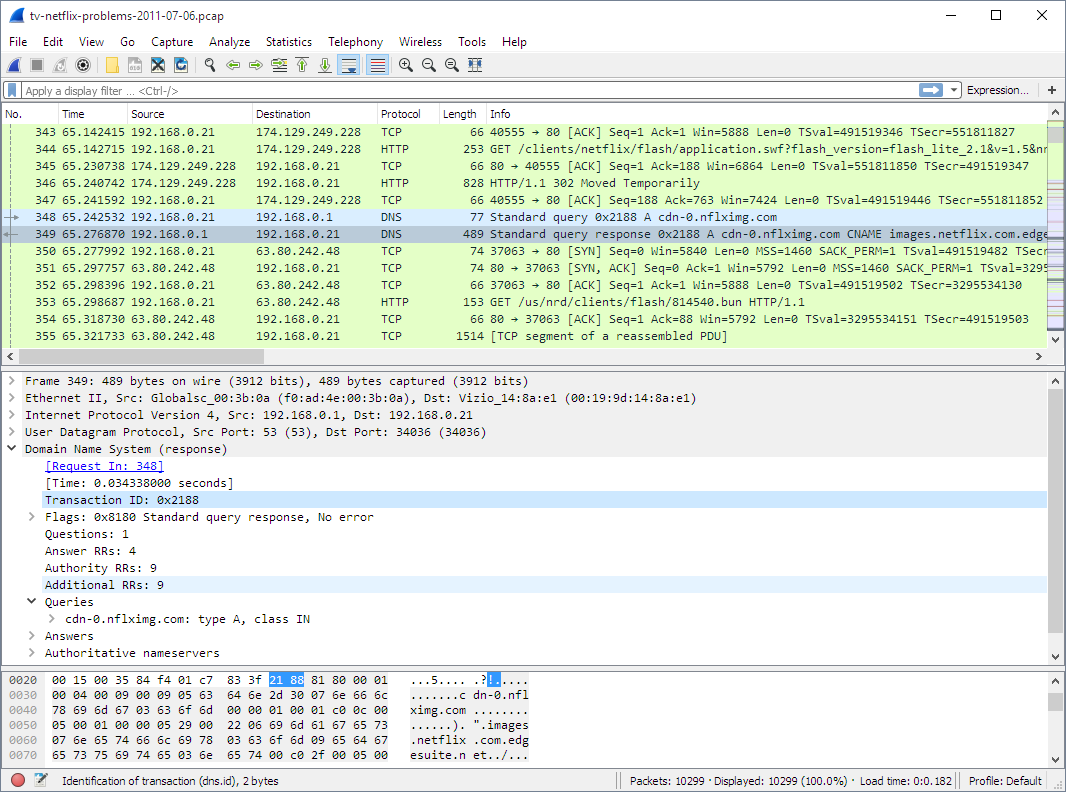
\includegraphics[width=1.0\textwidth]{Immagini/wireshark_dashboard.png}
            \caption{Pannello di controllo Wireshark\footref{wireshark_site}.}
            \label{fig:wireshark_dashboard}
        \end{figure}

    \subsection{SNMP Network Monitoring}
        Il Simple Network Management Protocol è un protocollo di management della rete molto utilizzato per sorvegliare i dispositivi nel network e i suoi sistemi. È un protocollo di rete che permette ai network administrator di raccogliere informazioni dai dispositivi nella rete, così da monitorare le loro performance e gestirli da remoto. Permette di raccogliere parametri importanti come la banda utilizzata, l'utilizzo di risorse hardware e la percentuale di errori. Fornisce una visione in real time dell'infrastruttura di rete e consente un troubleshooting proattivo. Per implementare questa tecnica di controllo, i dispositivi devono avere un software con un agente SNMP installato così da poter fornire dati all'SNMP manager. Questa tipologia di monitoring offre diverse funzionalità utili agli amministratori della rete per gestire la rete. Il device discovery permette di scoprire i dispositivi nella rete in automatico, semplificando il processo di aggiunta dei dispositivi al sistema di monitoring. Permette anche di rilevare anomalie nei dispositivi collegati alla rete generando notifiche e alert per permettere una risposta pronta in situazione critiche. Grazie agli agenti precedentemente menzionati è anche possibile modificare le configurazioni dei dispositivi anche da remoto, garantendo una gestione più facile e rapida su più device, assicurando una coesione ai standard della rete \cite{obkio_net_monitors}. Uno dei software utilizzati dalle grandi aziende è Obkio\footnote{\label{obkio_site}Sito: (\url{https://obkio.com/})}.

        \begin{figure}[H]
            \centering
            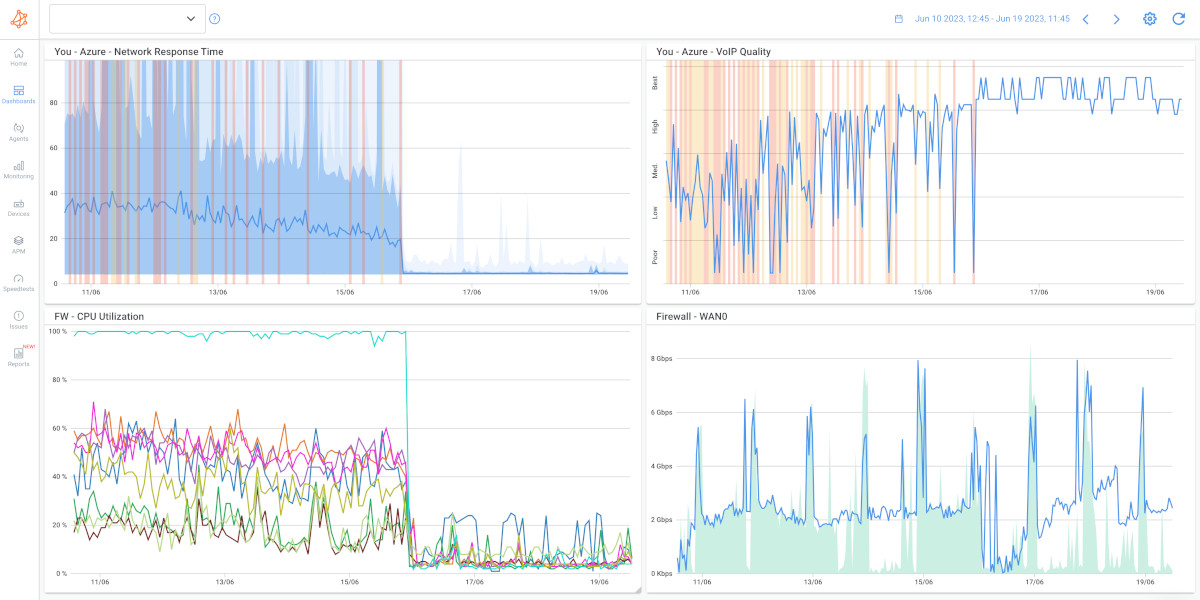
\includegraphics[width=0.9\textwidth]{Immagini/obkio_dashboard.jpg}
            \caption{Pannello di controllo Obkio\footref{obkio_site}.}
            \label{fig:obkio_dashboard}
        \end{figure}


    \subsection{SIEM}
        Per gestire e poter utilizzare tutte le informazioni, gli alert e i dati provenienti dal monitoring della rete è necessario un sistema di \textbf{Security Information and Event Management}, SIEM. Questo strumento raccoglie tutti i dati e gli eventi relativi alla sicurezza da diverse fonti di una rete, i quali sono rappresentati tramite schemi diversi, spesso prioritari di qualche brand. I SIEM includono anche informazioni di contesto che possono essere utili nell'analisi, come dati aggiornati sugli asset aziendali, regole e priorità degli alert. Il compito di questo sistema è quello di correlare tra loro i log provenienti da fonti diverse, trovando attributi comuni così da poter definire un pattern per degli attacchi o scenari che possono allertare i Security Analists. I SIEM lavorano con gli strumenti di monitoring definiti in precedenza e utilizzano vari sensori e applicazioni presenti sui dispositivi e nella rete per monitorare il comportamento di questi, se necessario inoltre archivia in un database eventi per cui potrebbe essere opportuna un'analisi a lungo termine, così da non tralasciare malware potenzialmente resilienti. 
        Vengono create delle regole generate algoritmicamente, le quali catturano informazioni su comportamenti malevoli, il rischio però è che se queste regole sono mal configurate si rischia di trasformare il SIEM in un sistema di big data, che renderebbe l'archiviazione, la ricerca, l'analisi e la condivisione una sfida. Un altro problema più importante riguarda quello dei falsi positivi; infatti, se le regole dovessero generare troppi falsi positivi tra gli allarmi, l'analisi degli eventi potrebbe diventare difficile da gestire. Allo stesso modo, un numero alto di falsi negativi potrebbe compromettere la rete; bisogna quindi trovare il giusto compromesso tra i due, così da poter individuare il maggior numero possibile di attacchi senza però raccogliere troppi dati inutili ai fini della sicurezza \cite{siem_and_soc_paper}.


        \begin{figure}[H]
            \centering
            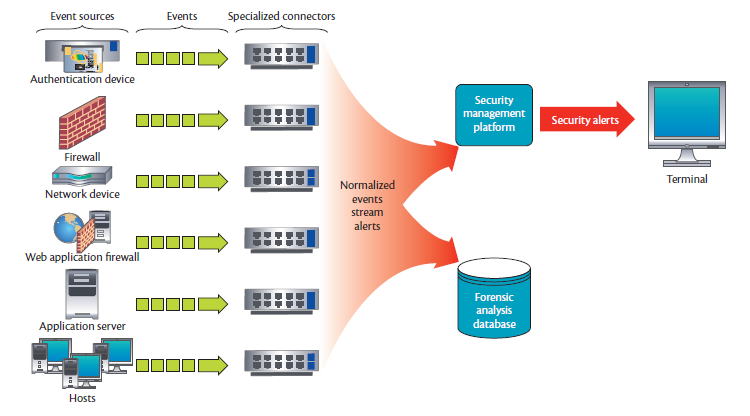
\includegraphics[width=1.0\textwidth]{Immagini/siem_paper_image.PNG}
            \caption{Un'architettura generica di un SIEM. Il SIEM accetta gli input dai vari dispositivi di sicurezza e sensori. Dopo averli ricevuti li normalizza in un formato comune~\cite{siem_and_soc_paper}.}
            \label{fig:siem_paper_image}
        \end{figure}
    
        Questo strumento è particolarmente utile nella manutenzione per riconoscere minacce in tempo reale, migliorare l'efficienza organizzativa, grazie a dashboard centrali che permettono una risposta rapida ed efficiente alle minacce e agli incidenti. Permette inoltre di condurre indagini forensi all'interno della rete, analizzando attività sospette e imparando da incidenti passati. Fornisce inoltre un grande supporto di sicurezza alla rete, mitigando e monitorando i BYOD, tracciando le attività di rete di tutti gli utenti, i dispositivi e le applicazioni, migliorando notevolmente la trasparenza dell'intera infrastruttura e rilevando le minacce indipendentemente da dove si accede agli asset \cite{siem_and_soc_paper}.

    \subsection{SOC}
        Per monitorare gli eventi, tutte le informazioni contenute nella rete e i suoi asset, avremmo bisogno di un \textbf{Security Operation Center}, SOC. Si tratta di un'infrastruttura dove risiede un team specializzato incaricato di monitorare, analizzare e rispondere agli incidenti della rete in tempo reale. Questo reparto riceve in continuazione informazioni sugli eventi dai sensori, dai log e dagli alert di cui abbiamo parlato in precedenza. Quando un alert viene azionato e notificato, il personale del SOC deve determinare se si tratta di un falso positivo o meno e il suo compito è quello di proteggere gli asset aziendali. Un SOC può essere in-house, e quindi interno all'organizzazione, o preso in out-sourcing, ossia appaltato a un'azienda esterna. In genere la seconda via è quella percorsa dalla maggior parte delle organizzazioni in quanto la prima risulta essere troppo costosa. Queste strutture possono essere fisiche o cloud-based e il personale che compone questa struttura è personale specializzato in sicurezza informatica \cite{soc_functions_book}. 
        Questa divisione ha diverse funzioni come il threat hunting e il threat intelligence, ossia il compito di fornire informazioni aggiornate sui rischi di cyber sicurezza moderni. Questa funzione permette anche di tenere il SOC, e di conseguenza l'organizzazione, in costante sviluppo per proteggersi. Il threat hunting consiste nell'identificare e investigare attivamente gli attacchi che potrebbero avere bypassato i controlli di sicurezza. Abbiamo poi una sezione che si occupa di mantenere gli strumenti utilizzati dal SOC e i suoi logs, assicurandosi il corretto funzionamento dell'organizzazione. Questa si occupa anche di gestire gli incidenti quando ci sono, ossia di investigarne la causa. Il loro obiettivo è mitigare l'impatto dell'attacco e questo viene anche segnalato al reparto che si occupa di Incident Management, che si occupa della parte gestionale dell'incidente. Un altro reparto importante in questa struttura è quello che gestisce le vulnerabilità; il loro compito è trovarle all'interno dell'organizzazione e questo compito richiede risorse, competenze e strumenti proprio per il pentesting. Troviamo poi la funzione di Insider Threat che si occupa di individuare gli attacchi provenienti dall'interno utilizzando tecniche e strumenti diversi rispetto agli attacchi esterni \cite{soc_functions_book}.

        \begin{figure}[H]
            \centering
            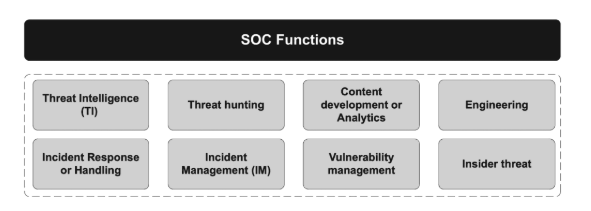
\includegraphics[width=1.0\textwidth]{Immagini/soc_functions.PNG}
            \caption{Descrizione delle funzionalità di un SOC \cite{soc_functions_book}.}
            \label{fig:soc_funcionts}
        \end{figure}

        Questa infrastruttura segue una struttura particolarmente gerarchica e divide infatti il proprio personale in analisti di sicurezza di diverso livello, che vanno in genere dall'uno, coloro che troviamo in prima fila che sorvegliano continuamente l'infrastruttura della rete aziendale, al terzo, che in genere corrisponde al CISO o al Cyber Security Manager di cui abbiamo parlato in precedenza. Per il SOC è fondamentale agire secondo dei framework e delle politiche di sicurezza prestabilite e ben delineate, manutenendosi secondo delle politiche di governance da rispettare. Un altro strumento di cui abbiamo parlato in precedenza e di cui il SOC ne fa ampio utilizzo è il SIEM.
        
        \newpage
        
        \begin{figure}[H]
            \centering
            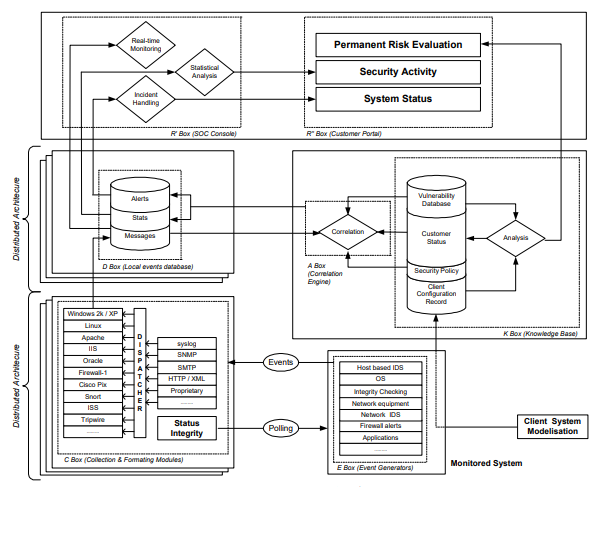
\includegraphics[width=0.99\textwidth]{Immagini/soc_architecture.PNG}
            \caption{Descrizione dell'architettura di un SOC \cite{soc_architecture_pic}.}
            \label{fig:soc_architecture}
        \end{figure}

        \subsubsection{MITRE ATT\&CK}
            Abbiamo citato in precedenza i Knowledge  Database, ossia delle banche dati dove sono raccolte tutte le tecniche e tattiche di attacco già conosciute, utili per poter prevenire e rilevare le offensive informatiche.
            Tra i Knowledge  Database più utilizzati troviamo il MITRE ATT\&CK, un database accessibile a tutti contenente la maggior parte degli attacchi conosciuti e in continuo aggiornamento per mitigare questo problema. Questo strumento funziona basandosi su una vasta Threat Intelligence Mapping, infatti grazie alle tattiche, tecniche e procedure (TTP), utilizzate in passato nei vari attacchi, si è in grado di prevedere il comportamento futuro di un attaccante, informazione fondamentale per poter difendersi al meglio. Questo è possibile grazie al continuo aggiornamento di questo strumento, ma anche grazie a una struttura organizzata delle TTP usate. Un'altra funzionalità chiave di questo strumento, chiamata Data Source Gap Identification, è un processo che identifica le lacune nei dati disponibili per rilevare tecniche specifiche. Il MITRE ATT\&CK elenca per ogni tecnica i data source necessari, come: log di processo, registri di autenticazione, dati di rete e altri, permettendo alle organizzazioni di valutare se dispongono degli strumenti per monitorare quelle attività \cite{MITRE_ATT_CK_description}.
        
    
           L'utilizzo del MITRE ATT\&CK può essere fondamentale nei SOC, in quanto fornisce la conoscenza necessaria per le loro operazioni base, ossia rilevare, rispondere e mitigare le minacce cibernetiche, fornendo conoscenze standardizzate e dettagliate per capire le tecniche e tattiche avversarie. Il framework è organizzato in diverse categorie, tra cui le tattiche. Queste rappresentano ad alto livello gli obiettivi a cui un attaccante mira. Ognuna di queste tattiche ha diverse tecniche che specificano i dettagli dei metodi usati per raggiungere l'obiettivo della tattica. Altri componenti del framework contengono le sotto-tecniche, che offrono metodi più dettagliati per gli obiettivi tattici di difesa, le procedure, che descrivono in maniera specifica che tipo di avversario applica certe tecniche o sotto-tecniche e le mitigazioni, che specificano misure difensive per prevenire la riuscita di un attacco.

             \begin{figure}[H]
                \centering
                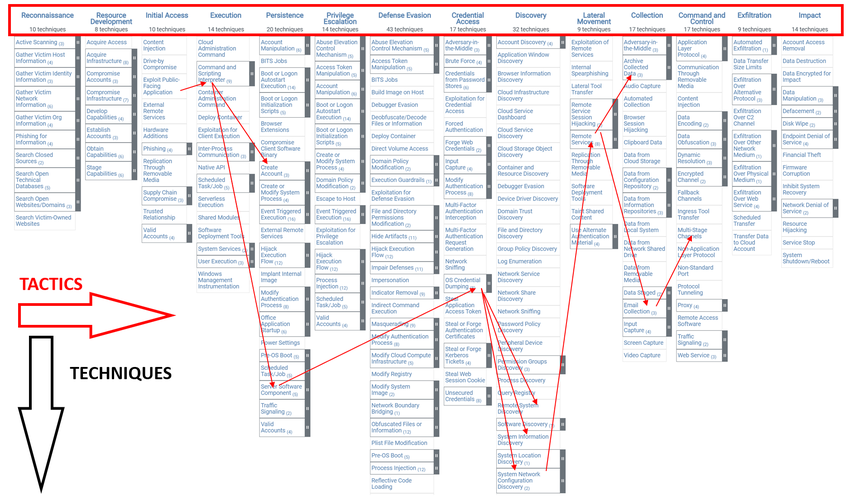
\includegraphics[width=1.0\textwidth]{Immagini/mitre_att_ck_matrix.png}
                \caption{Il layout della matrice del MITRE ATT\&CK per il dominio Enterprise\protect\footnotemark. Le tattiche sono organizzate per colonne mentre le tecniche per righe \cite{mitre_attck_matrix_pic_paper}.}
                \label{fig:mitre_att_ck_matrix}
            \end{figure}
           \footnotetext{Il termine dominio Enterprise si riferisce a un insieme di sistemi, reti e tecnologie utilizzate all'interno di organizzazioni aziendali o imprese.}

            Grazie a questo strumento i SOC hanno un aiuto per allineare le loro strategie anche in base alle potenziali intenzioni di un attaccante, aumentando l'efficienza e la risposta alle minacce della cyber sicurezza e tenendosi sempre aggiornati in materia, permettendo di reagire proattivamente alla minaccia.
           In un campo in continuo cambiamento come la cyber security è cruciale per i Security Operation Centers capire le tattiche e le tecniche avversarie per sviluppare una strategia di risposta funzionale. Vediamo come in questi paper \cite{paper_esempi_concreti_diminuzione_danni_potenziali_n3}, \cite{paper_esempi_concreti_diminuzione_danni_potenziali_n4} l'integrazione di questo knowledge database ha migliorato le strategie dei SOC, i paper forniscono esempi concreti di come lo strumento ha minimizzato i potenziali danni e perdite. Migliorando anche i rapporti di rilevazione e abbassando i tempi di risoluzione degli incidenti. Ricordiamo che questo strumento si basa sugli attacchi già conosciuti, è quindi fondamentale non utilizzare questo come unica risorsa di difesa, rendendo comunque fondamentale l'allocazione di risorse per la formazione del personale e di altri strumenti necessari per combattere le minacce \cite{mitre_attck_matrix_pic_paper}.
        
\section{Manutenzione Preventiva}
    La manutenzione preventiva consiste in un approccio cautelare nei confronti degli asset digitali dell'organizzazione e delle sue infrastrutture, cercando di prevenire, appunto, violazioni nella rete. Questa è una strategia che sta acquistando sempre più importanza tra le società. Grazie alla prevenzione, tramite strumenti come il controllo degli accessi, il patch management, i backup, e altri, si è in grado di rispondere meglio agli attacchi e di fornire continuità ai servizi o alle risorse in maniera più rapida. Questa tecnica cerca quindi di identificare e correggere i potenziali problemi prima che si trasformino in vulnerabilità o incidenti. Un punto chiave della manutenzione preventiva è anche la formazione del personale. Mettere in guardia e informare i propri dipendenti dei pericoli a cui l'infrastruttura di rete è soggetta, li potrà aiutare a riconoscere e a rispondere a comportamenti pericolosi. A differenza della manutenzione classica, quella preventiva permette dei down time minori, ma previene anche potenziali perdite di dati e violazioni di sicurezza.

    \subsection{Controllo degli Accessi}
        Uno dei metodi più antichi di prevenzione è il controllo degli accessi. Il compito di questa funzione di sicurezza è quello di limitare le attività di utenti legittimi. Tramite un reference monitor\footnote{Fonte: Wikipedia (\url{https://en.wikipedia.org/wiki/Reference_monitor})} controlliamo i tentativi di accesso da parte di un utente (o un programma eseguito da un utente) verso un oggetto nel sistema. Il reference monitor consulta un database di autorizzazioni per determinare se un utente può effettivamente fare un'operazione o meno. Le autorizzazioni in questo database sono gestite da un security administrator\footnote{Fonte: Wikipedia (\url{https://it.wikipedia.org/wiki/Sistemista})} basandosi sulle policy interne di sicurezza dell'organizzazione. È importante distinguere l'autenticazione dal controllo degli accessi, infatti stabilire correttamente l'identità di un utente è responsabilità dei servizi di autenticazione mentre il controllo degli accessi prende per buona l'identità dell'utente in quanto non è di sua competenza. Notiamo inoltre che in una rete il processo di autenticazione è più difficile da gestire in quanto un potenziale intruso potrebbe osservare il traffico del network e può replicare i protocolli di autenticazione per mascherarsi come utente legittimo, attacco noto come masquerade attack.
        Dobbiamo fare una distinzione anche tra politiche e meccanismi di sicurezza. Le politiche sono linee guida di alto livello che determinano come vengono controllati gli accessi e come vengono prese le decisioni di accesso. I meccanismi sono funzioni software e hardware di basso livello che possono essere configurate per implementare una politica. In generale non esistono politiche migliori di altre in quanto alcune potrebbero essere adatte per un sistema ma non per un altro. Negli anni sono state sviluppate diverse idee astratte per implementare questa funzionalità, come la matrice degli accessi. Alla base di queste idee troviamo sempre una divisione tra oggetti e soggetti. Gli oggetti sono i dati che troviamo memorizzati in un sistema, la cui protezione è il requisito fondamentale, mentre le entità che iniziano delle attività sono chiamati soggetti, ossia utenti o programmi eseguiti da utenti. Un utente si autentica al sistema con soggetti differenti in occasioni differenti in base al tipo di privilegio di cui ha bisogno. Il soggetto inizia quindi operazioni sugli oggetti che saranno permesse o meno in base alle autorizzazioni prestabilite nel sistema.
        
        \begin{figure}[H]
                \centering
                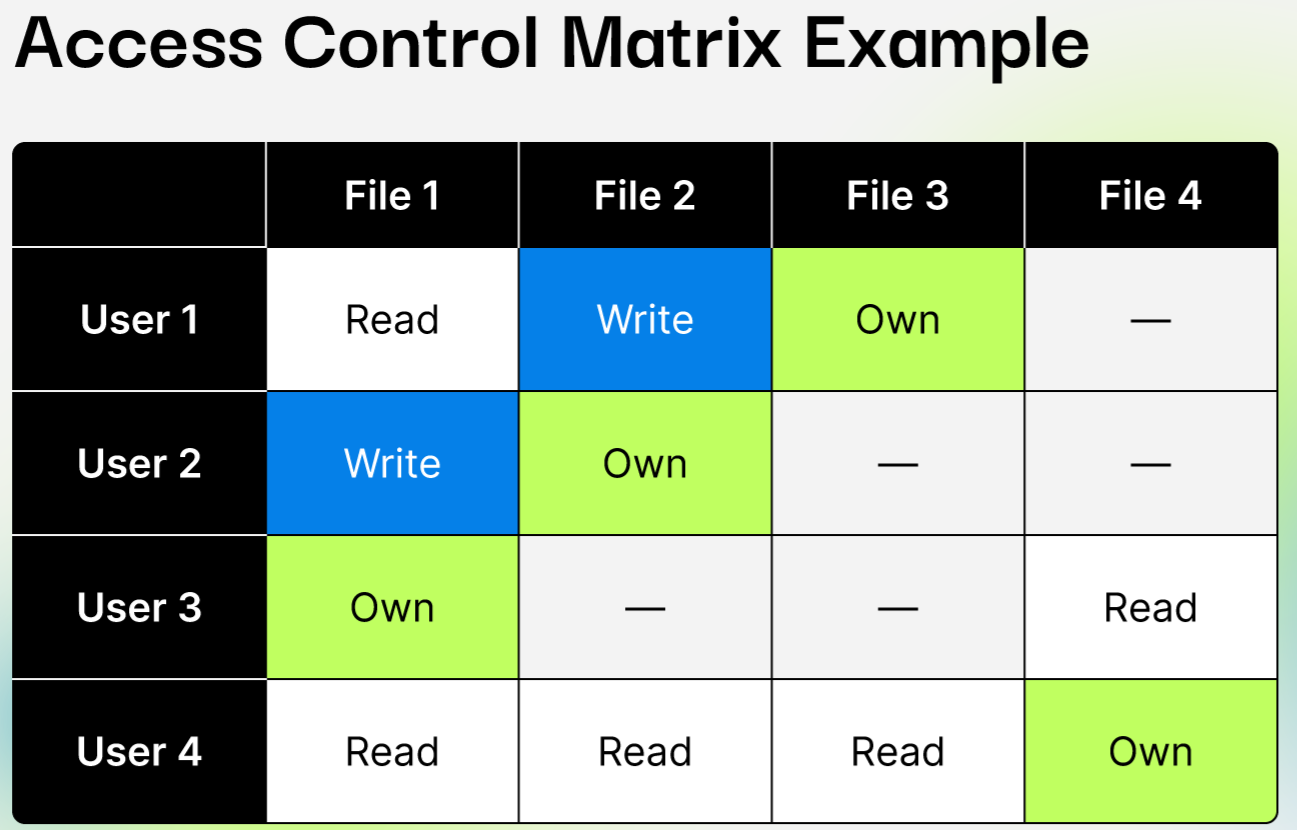
\includegraphics[width=0.8\textwidth]{Immagini/access-control-matrix.png}
                \caption{Un esempio di matrice di controllo degli accessi con i suoi permessi \cite{access_control_matrix_pic}.}
                \label{fig:access_matrix}
            \end{figure}

        In questo modello concettuale troviamo delle righe per ogni soggetto e delle colonne per ogni oggetto e ogni cella della matrice specifica i permessi di accesso per ogni soggetto nella riga e ogni oggetto nella colonna.

        Le autorizzazioni sono espresse in termini di diritti di accesso e dipendono dal tipo di oggetto in questione, per i file i diritti di accesso saranno “read”, “write”, “execute” e “own”, in particolare l'attributo di proprietà può controllare chi può cambiare i diritti di accesso per il file. Se l'oggetto dovesse essere per esempio un conto bancario i diritti saranno tipo “inquiry”(consultare), “credit”(accreditare) e “debit”(addebitare) che corrisponderanno alle operazioni basiche che possono essere effettuate su un conto.

        Dato che nei sistemi reali una matrice di questo tipo avrebbe dimensioni enormi, si è pensato a degli approcci implementativi diversi.

        \subsubsection{Access Control List - ACL}
             Ogni oggetto è associato a una ACL, che specifica, per ogni soggetto nel sistema, gli accessi che il soggetto è autorizzato a eseguire sull'oggetto. Questo approccio si limita quindi a memorizzare le colonne della matrice precedentemente menzionata. Guardando all'ACL di un oggetto, è facile determinare gli attributi per cui un soggetto è attualmente autorizzato. Questo ha però lo svantaggio di rendere difficile la determinazione di tutti gli accessi che un soggetto ha; sarebbe infatti necessario analizzare l'ACL di tutti gli oggetti nel sistema in base a un particolare soggetto. Allo stesso modo, per rimuovere tutti i permessi per un particolare utente, tutti gli ACL dovrebbero essere analizzati; nella realtà si fa prima a eliminare l'istanza dell'utente corrispondente, anche se questo non si applica se è necessaria solo la modifica di alcuni permessi per un utente, rendendola comunque un'operazione complessa.

             \begin{figure}[H]
                \centering
                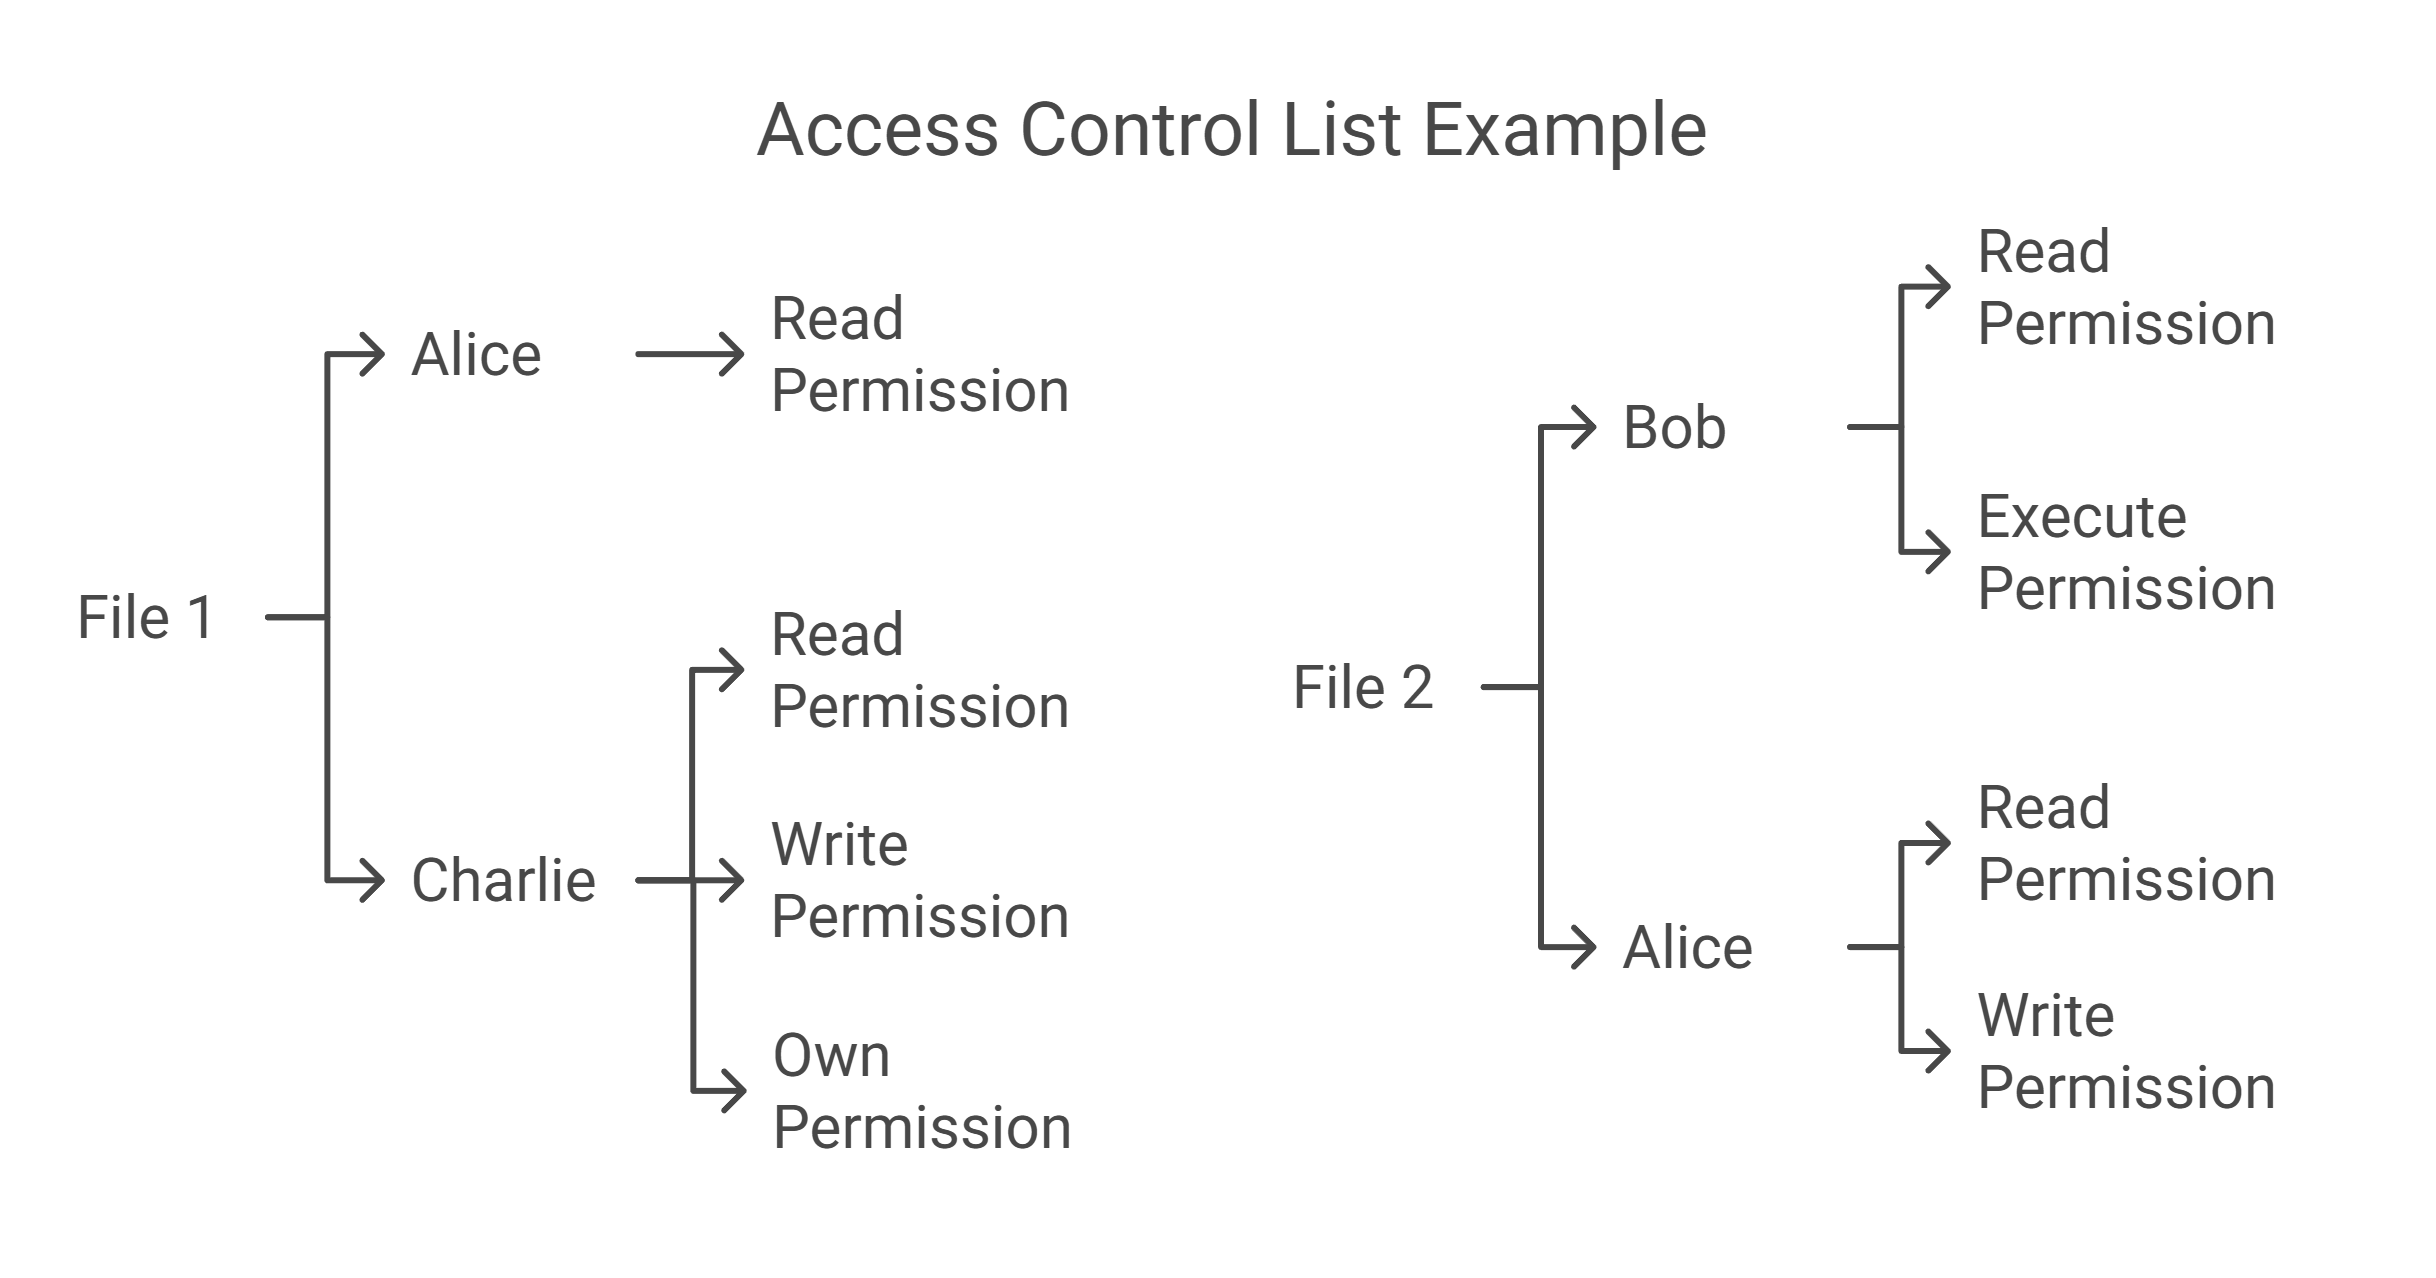
\includegraphics[width=0.67\textwidth]{Immagini/access-control-list.png}
                \caption{Rappresentazione concettuale di controllo degli accessi tramite ACL con i suoi permessi.}
                \label{fig:acl_pic}
            \end{figure}
             
        \subsubsection{Capabilities}
            L'approccio delle capability list è il duale dell'access control list, dove ad ogni soggetto è associato con una lista, chiamata  capability list, che indica per ogni oggetto nel sistema quale attributo un determinato soggetto possiede per quell'oggetto. In questo tipo di approccio è più facile analizzare tutti gli attributi di un utente analizzando la  capability list di questo, allo stesso modo determinare tutti i soggetti che possono accedere a un particolare oggetto richiede l'analisi di ogni capability list di ogni soggetto.

            È possibile combinare i metodi di ACL e di Capabilities, infatti in sistemi distribuiti questo comporta il vantaggio di non dover ripetere l'autenticazione di un utente in base al tipo di operazioni che deve compiere, permettendo al soggetto di autenticarsi una sola volta e di ottenere le sue capability list e di ottenere i servizi dai vari server nel sistema e se sono necessari ulteriori permessi ogni server può fornire l'ACL. Lo svantaggio di questo approccio varia in base all'ordine logico della tabella dei permessi, infatti se questa è ordinata in base ai soggetti otteniamo i vantaggi della capability list, altrimenti delle ACL.

            \begin{figure}[H]
                \centering
                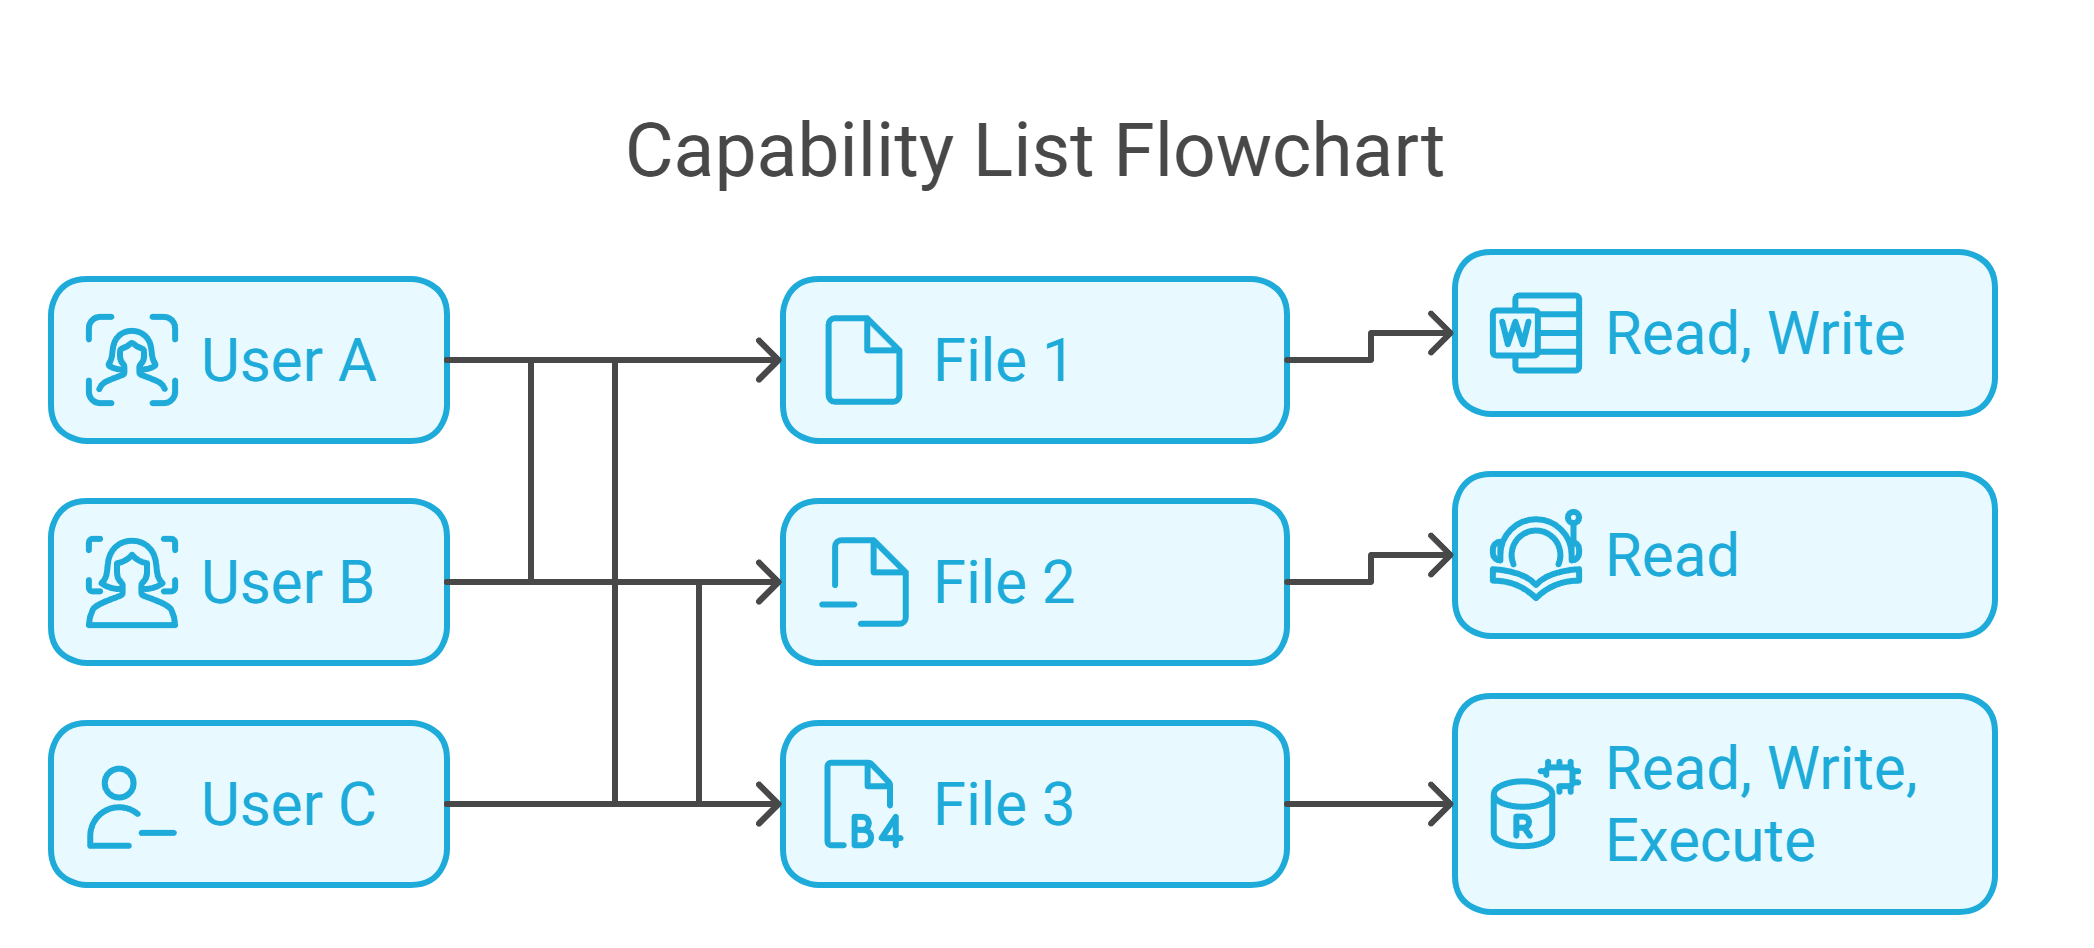
\includegraphics[width=0.67\textwidth]{Immagini/capability_list.png}
                \caption{Rappresentazione di un esempio di controllo degli accessi tramite capabilities con i suoi permessi.}
                \label{fig:cap_pic}
            \end{figure}
            
    \subsection{Policies di Controllo degli Accessi}
        Analizziamo ora 3 tipi di policy di controllo degli accessi più utilizzate. Alcune policies sono categorizzate in discretionary e non-discretionary, o mandatory.

        \subsubsection{Classical Discretionary Policies - DAC}
            Le classical discretionary policies, anche chiamate \textbf{DAC}, regolano l'accesso degli utenti alle informazioni sulla base dell'identità dell'utente e delle autorizzazioni che specificano, per ogni utente, o gruppo di utenti, e per ogni oggetto nel sistema, gli attributi di accesso (“read”, “write” e “execute”) consentiti all'utente sull'oggetto. Ogni richiesta di accesso a un oggetto da parte di un utente viene verificata rispetto alle autorizzazioni definite. Se esiste un'autorizzazione che stabilisce che l'utente può accedere all'oggetto nella modalità specificata, l'accesso viene concesso; in caso contrario, viene negato.

            Tuttavia, queste politiche di controllo degli accessi presentano lo svantaggio di non garantire un controllo effettivo sul flusso delle informazioni all'interno di un sistema. È semplice aggirare le restrizioni di accesso definite tramite le autorizzazioni. Ad esempio, un utente in grado di leggere dati può condividerli con altri utenti non autorizzati, senza che il proprietario ne sia a conoscenza. Ciò accade perché le politiche discrezionali non impongono alcuna restrizione sull'utilizzo delle informazioni da parte di un utente dopo che quest'ultimo le ha ottenute, ovvero la diffusione delle informazioni non è controllata. Questo problema non lo troviamo nelle politiche di accesso di tipo mandatory, che vedremo dopo.

            Inoltre, dato che sono basate su autorizzazioni esplicitamente specificate, sono definite chiuse, le quali garantiscono l'accesso solo se esiste un riscontro positivo con le autorizzazioni, altrimenti viene negato. Concetto simile a quello del whitelisting. Politiche opposte, chiamate aperte, negano l'accesso se esiste un divieto nelle autorizzazioni, come una sorta di blacklisting. Ogni richiesta di accesso da parte di un utente viene verificata rispetto alle autorizzazioni negative definite e viene concessa solo se non esistono autorizzazioni che negano l'accesso.

            Questo tipo di politiche sono basate su ACL o Capabilities.
            
        \subsubsection{Classical Mandatory Policies - MAC}
            Le Classical Mandatory Policies, anche chiamate MAC, regolano l'accesso sulla base della classificazione di soggetti e oggetti nel sistema. A ogni utente e oggetto del sistema viene assegnato un livello di sicurezza, chiamato “sensitivity label”. Il livello di sicurezza associato a un oggetto riflette la sensibilità delle informazioni in esso contenute, ossia il potenziale danno derivante dalla loro divulgazione non autorizzata. Il livello di sicurezza associato a un utente, denominato anche “clearance”, riflette l'affidabilità dell'utente nel non divulgare informazioni sensibili a utenti non autorizzati ad accedervi. L'accesso a un oggetto da parte di un soggetto è permesso solo se qualche relazione tra i loro livelli di sicurezza è soddisfatta.

            Per garantire il corretto flusso delle informazioni, sono richiesti due principi fondamentali:

            \begin{itemize}
                \item \textbf{Read Down}: la clearance del soggetto deve dominare il livello di sicurezza dell'oggetto che si desidera leggere.
                \item \textbf{Write Up}: la clearance del soggetto deve essere dominata dal livello di sicurezza dell'oggetto che si desidera scrivere.
            \end{itemize}

            Il rispetto di questi principi impedisce che informazioni contenute in oggetti di livello alto (quindi più sensibili) possano fluire verso oggetti di livello più basso, consentendo di fatto solo un flusso di informazioni verso l'alto (o all'interno della stessa classe di sicurezza). È importante anche comprendere la relazione tra utenti e soggetti in questo contesto. Per esempio se l'utente umano Bell ha una clearance di livello S (Secret), e si autentica sempre come un soggetto S, questo soggetto non potrà leggere gli oggetti TS (Top Secret), a causa della regola read down, però con la regola write up ci sono due aspetti che possono sembrare contro intuitivi all'inizio. Infatti lo stesso soggetto potrà scrivere sugli oggetti TS, anche se non può leggerli. Molti sistemi a causa di questo inconveniente non consentono la regola di write up, limitando i permessi di scrittura allo stesso livello del soggetto. La regola write up è stata pensata per poter permettere agli utenti di livelli inferiori di interfacciarsi con quelli di livelli superiori. Notiamo come questo tipo di regole non permette il contrario, infatti i soggetti con permessi superiori non possono interagire con quelli con permessi inferiori, per farlo devono registrarsi come soggetti con permessi inferiori. Qual è quindi l'utilità di queste restrizioni?
    
            Questa implementazione è la FSM Bell-LaPadula, questo modello è stato sviluppato per essere utilizzato nel dipartimento della difesa americano\footnote{Fonte: Wikipedia (\url{https://en.wikipedia.org/wiki/United_States_Department_of_Defense})}. Questo modello considera infatti più sicuri gli umani e previene il leak di informazioni da parte di software malevoli dai livelli superiori a quelli inferiori.

             Il MAC può essere applicato anche per la protezione dell'integrità delle informazioni. Ad esempio, i livelli di integrità potrebbero essere Cruciale (C), Importante (I) e Sconosciuto (U). Il livello di integrità associato a un oggetto riflette il grado di fiducia che può essere riposto nelle informazioni in esso memorizzate, nonché il potenziale danno derivante da modifiche non autorizzate a tali informazioni. Il livello di integrità associato a un utente riflette l'affidabilità dell'utente nell'inserire, modificare o eliminare dati e programmi a quel livello. Principi analoghi a quelli definiti per la segretezza devono essere rispettati, come segue:
             \begin{itemize}
                 \item \textbf{Read Up}: Il livello di integrità di un soggetto deve essere dominato dal livello di integrità dell'oggetto che viene letto.
                 \item \textbf{Write Down}: Il livello di integrità di un soggetto deve dominare il livello di integrità dell'oggetto che viene scritto.
             \end{itemize}
            Notiamo quindi che l'essenza del MAC è il flusso di informazioni unidirezionale in una rete di etichette di sicurezza.

\newpage

        \subsubsection{Role-Based Policies - RBAC}
            Questo tipo di policy, \textbf{RBAC}, nasce per un'esigenza di soddisfare le aziende private. Questo tipo di policy per il controllo degli accessi è di tipo MAC e definisce condizioni specifiche per l'accesso a un oggetto.
                Queste politiche consentono di specificare le autorizzazioni da concedere agli utenti (o ai gruppi) sugli oggetti, come nell'approccio discrezionale, combinando tale possibilità con la definizione di restrizioni, simili a quelle dell'approccio MAC, sull'assegnazione o sull'utilizzo di tali autorizzazioni. Le politiche role-based regolano l'accesso degli utenti alle informazioni in base alle attività che questi svolgono nel sistema. Tali politiche richiedono l'identificazione di ruoli all'interno del sistema. Un ruolo può essere definito come un insieme di azioni e responsabilità associate a una specifica attività lavorativa. Invece di specificare tutti gli accessi che ciascun utente è autorizzato a eseguire, le autorizzazioni di accesso sugli oggetti sono specificate per i ruoli. Agli utenti vengono assegnate le autorizzazioni per assumere determinati ruoli. Vediamo come in questo studio del NIST conferma che i ruoli rappresentano un approccio utile per molte organizzazioni commerciali e governative \cite{nist_study_rbac}.

                L'utente che assume un determinato ruolo è autorizzato a eseguire tutte le operazioni per cui quel ruolo è abilitato. In generale, un utente può ricoprire ruoli diversi in momenti diversi. Inoltre, lo stesso ruolo può essere assegnato a più utenti, anche contemporaneamente. Alcune implementazioni sul controllo degli accessi basato sui ruoli permettono a un utente di svolgere più ruoli in contemporanea, mentre altre limitano l'utente a un solo ruolo alla volta o stabiliscono che alcuni ruoli possano essere combinati, mentre altri devono essere esercitati in modo esclusivo. Non esistono standard consolidati in questo ambito, quindi è probabile che diversi sistemi adottino approcci differenti.

                L'approccio basato sui ruoli offre numerosi vantaggi come: i \textbf{ruoli gerarchici}, in molti contesti esiste una gerarchia naturale di ruoli, basata sui principi familiari di generalizzazione e specializzazione. Questi semplificano ulteriormente la gestione delle autorizzazioni. Garantiscono inoltre l'accesso con il \textbf{minor privilegio} necessario per il compito da svolgere. Gli utenti autorizzati a ruoli potenti non hanno bisogno di esercitarli fino a quando quei privilegi non sono effettivamente necessari. Questo riduce al minimo il rischio di danni causati da errori involontari o da intrusi che si spacciano per utenti legittimi. La \textbf{separazione dei compiti}, ossia quel principio per cui nessun utente dovrebbe avere abbastanza privilegi da poter abusare del sistema autonomamente. Ad esempio, la persona che autorizza un assegno non dovrebbe essere la stessa che lo prepara. La separazione dei compiti può essere applicata in modo statico, ossia con ruoli che non possono essere eseguiti dallo stesso utente, o dinamico, applicando il controllo al momento dell'accesso. Un esempio di separazione dinamica dei compiti è la regola dei due responsabili. Il primo utente che esegue un'operazione che richiede due persone può essere qualsiasi utente autorizzato, mentre il secondo utente deve essere un altro utente autorizzato, diverso dal primo. Le politiche basate sui ruoli forniscono una classificazione degli utenti in base alle attività che svolgono. Allo stesso modo, dovrebbe essere fornita una classificazione per gli oggetti. Dando un esempio, generalmente un impiegato avrà bisogno di accedere ai conti bancari, mentre una segretaria avrà accesso a lettere e memo (o a un sottoinsieme di essi). Gli oggetti possono essere classificati in base al loro tipo (come lettere, manuali, ecc...) o al loro ambito di applicazione (lettere commerciali, lettere pubblicitarie, e così via). Le autorizzazioni di accesso per ruoli dovrebbero quindi essere basate sulle \textbf{classi di oggetti}, piuttosto che sugli oggetti specifici. Riprendendo l'esempio, al ruolo di segretaria può essere concessa l'autorizzazione a leggere e scrivere l'intera classe delle lettere, invece di fornire autorizzazioni esplicite per ciascuna singola lettera. Questo approccio ha il vantaggio di rendere l'amministrazione delle autorizzazioni molto più semplice e meglio controllata.
            
    \subsection{Patch Management}
        Negli anni si ha avuto un costante sviluppo della tecnologia e con questa anche di malware e vulnerabilità. Nasce quindi la necessità di un rilascio costante di aggiornamenti software, per fare in modo di proteggere i propri strumenti, hardware o software, da vari attacchi, sempre più nuovi. Ogni organizzazione deve stabilire una policy di gestione degli aggiornamenti e fare in modo che essa venga seguita. Questo processo consiste nell'applicazione degli aggiornamenti rilasciati dal fornitore per chiudere le vulnerabilità di sicurezza e ottimizzare le prestazioni di software e dispositivi. La gestione delle patch è talvolta considerata parte della gestione delle vulnerabilità ed è  fondamentale nella sicurezza della rete per impedire agli hacker di sfruttare le potenziali vulnerabilità presenti nei software per poi compromettere l'azienda \cite{ibm_patch_management_site}. Secondo dei dati dell'FBI e dell'università Carnegie Mellon, più del 90\% degli attacchi sono portati a termine tramite una vulnerabilità software causata da un mancato aggiornamento \cite{libro_patch_management}.

        Con infrastrutture di rete sempre più complesse nasce il bisogno di un sistema di aggiornamento adeguato, dato che le patch sono fondamentali nel mondo IT in quanto migliorano non solo la sicurezza ma anche le prestazioni e la produttività.
        Gli aggiornamenti possono infatti essere di vario tipo:
        \begin{itemize}
            \item \textbf{Aggiornamenti di Sicurezza}. Si focalizzano sul mettere in sicurezza i software, risolvendo vulnerabilità prima non note. Questo è uno dei punti di ingresso principali nella rete da parte degli hacker e il mancato aggiornamento può lasciare una porta di ingresso aperta per loro.
            \item \textbf{Aggiornamenti delle Funzionalità}. Questo tipo di patch punta a migliorare i software rilasciando nuove funzionalità.
            \item \textbf{Correzioni di Bug}. Queste correzioni risolvono problemi minori nell'hardware o nel software, in genere questi non causano problemi di sicurezza ma influiscono comunque sulle prestazioni.
        \end{itemize}

        Uno degli eventi più importanti nella storia della cyber security che ricordiamo ancora oggi e che porta alla luce l'importanza di questo argomento è stato l'attacco WannaCry del 2017, che sfruttando una vulnerabilità nella funzionalità SMB\footnote{Fonte: Wikipedia (\url{https://it.wikipedia.org/wiki/Server_Message_Block})} di Windows, che fu corretta da Microsoft il 14 Marzo 2017, e quindi prima della diffusione che datiamo al 14 Aprile 2017, quando fu scoperta e pubblicata dall'NSA~\cite{eternalblue_wiki}. Questo worm si diffuse però proprio per la negligenza in diversi computer non aggiornati, creando il panico in sistemi, anche critici, nella nostra società. A partire da quel momento venne presa molto più seriamente l'operazione di patch management.

        Le case produttrici hanno iniziato a rilasciare aggiornamenti più velocemente rispetto a prima per cercare di combattere la rapidità con cui gli exploit vengono diffusi al giorno d'oggi. Basta guardare a questo esempio, dove Microsoft \cite{windows_63_fixes_one_patch} ha rilasciato un aggiornamento per “fixare” 63 vulnerabilità nei suoi vari applicativi, oppure ad esempi come \cite{critical_azure_ai} e \cite{privilege_esc_cisco}, dove due case costruttrici hanno trovato vulnerabilità critiche\footnote{Fonte: NIST - NVD (\url{https://nvd.nist.gov/vuln-metrics/cvss})} nei loro prodotti. 

        Ci viene da chiederci quindi, se quindi siamo consapevoli di questi rischi, perché tali problemi ci sono ancora oggi e continuano ad essere sfruttati?
        
        La risposta è più complessa di quello che si può pensare, infatti  i reparti IT operano spesso in condizioni di carenza di personale e sovraccarico, divisi tra manutenzione ordinaria, supporto tecnico e emergenze. Gestire l'applicazione di patch su migliaia di dispositivi, anche diversi, considerando il flusso incessante di aggiornamenti settimanali, supera le capacità umane quando affidata esclusivamente a processi manuali; inoltre, in alcuni sistemi, con il passare del tempo, sono state applicate talmente “toppe” che la sola idea di introdurre una qualunque modifica suscita timore e incertezza tra il personale di supporto. L’inserimento di una nuova patch, infatti, rischia di causare più problemi di quanti ne risolva. Non esiste poi una soluzione unitaria per tutti i tipi di business ed è anche per questo motivo che il patch management è diventato un problema sempre più gravoso per le aziende~\cite{libro_patch_management}. Un altro fattore da considerare è che i fornitori spesso smettono di supportare le versioni più vecchie dei propri prodotti: ciò implica che non verranno più rilasciate patch per le nuove vulnerabilità, rendendo queste versioni meno sicure con il passare del tempo \cite{nist_patch_management}.

        Un programma efficace di gestione delle patch si articola in più fasi. Il numero di fasi può variare da un'azienda all'altra in base alla sua infrastruttura IT e ad altri fattori chiave, come la dimensione, la diversità nelle piattaforme, nei sistemi e nelle applicazioni, il livello di automazione e aggiornamento, la centralizzazione o decentralizzazione dell'IT e la disponibilità di risorse.
        
        Riprendiamo ora dal paper del NIST \cite{nist_patch_management}, sulla guida al patch management per le aziende, l'importanza di questa pratica e capiamo che la gestione delle patch è il processo di identificazione, acquisizione, installazione e verifica delle patch per prodotti e sistemi. Le patch correggono problemi di sicurezza e funzionalità nel software e nel firmware. Dal punto di vista della sicurezza, le patch sono di particolare interesse poiché contribuiscono a mitigare le vulnerabilità causate da difetti nel software; l'applicazione delle patch per eliminare queste vulnerabilità riduce significativamente le opportunità di ingresso. Inoltre, le patch sono generalmente il metodo più efficace per mitigare le vulnerabilità dei difetti nel software e spesso rappresentano l'unica soluzione pienamente efficace \cite{nist_patch_management}.

\newpage

            \subsubsection{Le difficoltà nel patch management - Tempistica, Priorità e Testing}

                La gestione delle patch aziendali ruota attorno a tre aspetti fondamentali: tempistiche, priorità e test. Installare immediatamente ogni nuova patch riduce la finestra di esposizione a eventuali vulnerabilità, ma le risorse limitate e i rischi operativi legati a patch non testate impongono di stabilire un ordine di priorità. Molti fornitori semplificano il processo rilasciando patch in “bundle” (ad esempio mensili o trimestrali), permettendo di effettuare i test e di distribuire gli aggiornamenti in un'unica soluzione. Ciò può però prolungare il tempo tra la scoperta di una vulnerabilità e il rilascio della patch, lasciando una finestra più ampia per eventuali attacchi, a meno che non si decida di pubblicare subito un aggiornamento urgente in caso di exploit attivo.

                Inoltre, il rilascio di una patch può fornire indicazioni utili agli aggressori, tramite reverse engineering, spingendo alcune organizzazioni a installarla immediatamente, anche senza test approfonditi, purché siano disponibili procedure di rollback (come gli snapshot di macchine virtuali). Va infine considerato che, per rendere effettive le patch, spesso è necessario riavviare servizi o interi sistemi, con un impatto diretto sulla continuità operativa. In definitiva, non conta solo quando la patch viene installata, ma quando diventa effettivamente operativa.

                Troviamo fondamentale per la  gestione delle patch a livello aziendale un inventario aggiornato e completo di software, applicazioni e sistemi operativi, installato su ogni host, incluse le versioni in uso. Senza queste informazioni, è impossibile identificare, reperire e installare correttamente le patch necessarie, oltre a rilevare eventuali versioni obsolete che richiedono aggiornamenti.

                L'installazione di una patch può generare effetti collaterali indesiderati. Ad esempio, può modificare inavvertitamente alcune impostazioni di sicurezza già presenti o introdurne di nuove, creando di fatto nuovi problemi di sicurezza proprio mentre si cerca di risolvere la vulnerabilità originaria.

                Una patch installata potrebbe non essere attiva finché il software non viene riavviato o modificato. Verificarne l'efficacia è complesso, soprattutto senza indicazioni chiare su eventuali riavvii richiesti. Testare la vulnerabilità è un'opzione rischiosa e fattibile solo se esiste già un exploit.

                \subsubsection{Tecnologie per il Patch Management Aziendale}
                
                Le tecnologie di patch management enterprise condividono un'architettura simile ad altre soluzioni di sicurezza: server centralizzati per gestione/reporting e console operative. Ciò che le differenzia è la metodologia di rilevamento delle patch mancanti, articolata in tre approcci: 
                \begin{itemize}
                    \item \textbf{Agent-Based}. Le tecnologie di patch management agent-based richiedono un agente installato su ciascun dispositivo, con server centrali che coordinano il processo. L'agente individua il software vulnerabile, scarica e applica le patch tramite privilegi amministrativi. Questo approccio è ideale per dispositivi remoti, come laptop o smartphone, grazie alla gestione decentralizzata.
                    
                    Le limitazioni di questo approccio possono essere, l'incompatibilità, come ad esempio per i sistemi embedded e il supporto limitato per dispositivi simili.
                    \item \textbf{Agentless Scanning}. Operano tramite server centrali che scansionano la rete per identificare patch mancanti, richiedendo privilegi amministrativi sui dispositivi per installare aggiornamenti e gestire riavvii. Il vantaggio principale è l'assenza di agenti installati localmente, semplificandone la gestione. Presentano alcune criticità come; i dispositivi remoti esclusi, tipo laptop in smart working, poiché non raggiungibili via rete locale, l'interferenza di rete: Firewall o NAT possono bloccare le scansioni, compromettendo l’accuratezza e il supporto limitato per piattaforme specializzate, analogamente alle soluzioni agent-based.
                    \item \textbf{Monitoraggio passivo della rete}. Analizzano il traffico locale per individuare applicazioni non aggiornati. A differenza delle soluzioni agent-based e agentless, questo approccio non richiede privilegi sui dispositivi, rendendolo ideale per monitorare sistemi non gestiti dall'organizzazione, come dispositivi di operatori esterni o visitatori. Questa tecnica offre un valore unico nel rilevare vulnerabilità “nascoste” e sistemi non gestiti, ma la sua efficacia è vincolata a contesti specifici. Per una copertura completa, è essenziale integrarlo con approcci agent-based e agentless, sfruttando i punti di forza di ciascuna metodologia in uno schema di difesa stratificato.
                \end{itemize}

                \begin{table}[H]  
                    \begin{center}  
                        \begin{tabular}{|P{40mm}|P{25mm}|P{25mm}|P{35mm}|}  
                            \hline  
                            \multicolumn{4}{|c|}{\textbf{Confronto delle Tecniche}} \\  
                            \hline  
                            \textbf{Caratteristica} & \textbf{Agent-Based} & \textbf{Agentless Scanning} & \textbf{Passive Network Monitoring} \\  
                            \hline  
                            Privilegi amministrativi richiesti sugli host? & Sì & Sì & No \vspace{8mm}\\  
                            \hline  
                            Supporta host non gestiti? & No & No & Sì \vspace{6mm}\\  
                            \hline  
                            Supporta host remoti? & Sì & No & No \vspace{4mm}\\  
                            \hline  
                            Supporta appliance? & No & No & Sì \vspace{2mm}\\  
                            \hline  
                            Larghezza di banda necessaria per la scansione? & Minima & Da moderata a eccessiva & Nessuna \vspace{10mm}\\  
                            \hline  
                            Possibile gamma di applicazioni rilevate? & Completa & Completa & Solo quelle che generano traffico non cifrato\\  
                            \hline  
                        \end{tabular}  
                        \caption{Confronto delle architetture \cite{nist_patch_management}.}  
                        \label{tab:confronto-tecniche}  
                    \end{center}  
                \end{table}  


\newpage                  

            \subsubsection{Capacità di Sicurezza e Gestione Operativa nelle Tecnologie di Patch Management}

                Le tecnologie di patch management rappresentano un pilastro critico nella difesa delle infrastrutture informatiche moderne, integrando tre dimensioni fondamentali: gestione dell'inventario, gestione delle patch e mitigazione dei rischi operativi. Centrali in questo contesto sono i protocolli come lo SCAP (Security Content Automation Protocol) \cite{scap_protocolsecurity}, che standardizzano l'organizzazione e l'analisi delle informazioni di sicurezza, garantendo coerenza e interoperabilità tra sistemi eterogenei.
                
                La gestione dell'inventario costituisce la base operativa, permettendo il rilevamento preciso del software installato, delle relative versioni e delle vulnerabilità associate. Le tecnologie di patch management sono progettate per identificare il software installato su ciascun host, comprese le versioni specifiche, con un focus prioritario sul rilevamento di quelle vulnerabili. Oltre alla mappatura, molte soluzioni integrano funzionalità avanzate per gestire il ciclo di vita del software: installare aggiornamenti, aggiungere/rimuovere componenti specifici, come plugin o librerie, o disinstallare intere applicazioni. Queste capacità le rendono strumenti polivalenti, non solo per la sicurezza ma anche per l'ottimizzazione delle risorse IT. Ovviamente, gli strumenti di patch management hanno diverse funzionalità, come: l'identificazione delle patch necessarie, il bundling e la prioritizzazione, la flessibilità operativa o l'installazione automatizzata e verifica.

                Dopo aver creato un sistema di patch management, i suoi amministratori devono testare, distribuire la soluzione e mantenere le sue operazioni e sicurezza.

                L'adozione di strumenti aziendali per il patch management, seppur potenzialmente portatrice di nuovi rischi, rappresenta una scelta strategica per mitigare minacce ben più gravi derivanti dall'inazione. Le organizzazioni che trascurano gli aggiornamenti sistematici espongono infatti i propri sistemi a vulnerabilità critiche, con conseguenze spesso catastrofiche. Gli strumenti di patching offrono un bilancio netto positivo: i benefici in termini di sicurezza superano ampiamente i rischi residui. I potenziali rischi possono essere: una patch alterata, credenziali utilizzate impropriamente, vulnerabilità nei componenti della soluzione, un'entità potrebbe monitorare le comunicazioni dello strumento per identificare vulnerabilità. Le organizzazioni devono ridurre questi rischi con tecniche che dovrebbero essere seguite quando si rilascia una qualsiasi applicazione critica per l'azienda.

                Le organizzazioni dovrebbero distribuire gli strumenti di patch management adottando un approccio a fasi, che consenta di affrontare problematiche procedurali e di comunicazione con un gruppo limitato di utenti prima di un rollout universale. Inizialmente, è comune focalizzarsi su sistemi standardizzati, come desktop omogenei e server farm a singola piattaforma con configurazioni simili. Una volta consolidata questa fase, è possibile affrontare contesti più complessi, come ambienti multi-piattaforma, desktop non standard, computer legacy o con configurazioni insolite. Per sistemi operativi, applicazioni non supportate da strumenti automatizzati o dispositivi con configurazioni particolari, tipo sistemi embedded, controlli industriali, dispositivi medici o sperimentali, potrebbe essere necessario ricorrere a metodi manuali. In tali casi, è essenziale definire procedure scritte e formalizzate per garantire un processo di patching manuale strutturato e tracciabile.

                Le società devono bilanciare sicurezza, usabilità e disponibilità operativa. 
                
                Ad esempio, le patch potrebbero compromettere altre applicazioni, problema mitigabile testandole prima del deployment. Forzare riavvii di applicazioni, OS o modifiche allo stato degli host può interrompere servizi o causare perdite di dati. È quindi cruciale equilibrare l'applicazione tempestiva delle patch con la necessità di mantenere la continuità operativa.

            \begin{figure}[H]
                \centering
                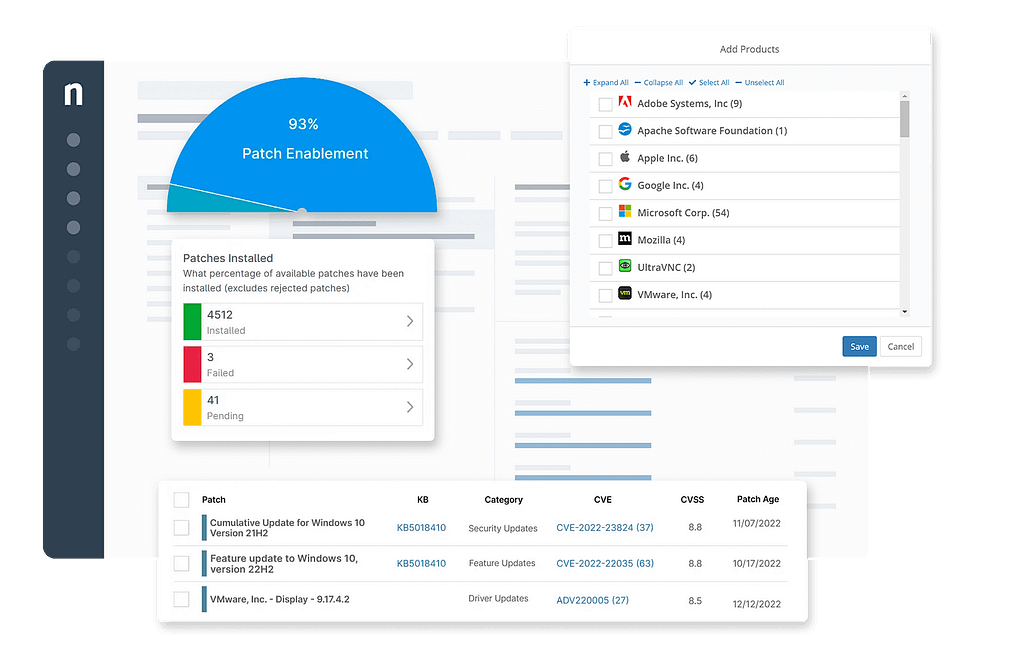
\includegraphics[width=1.0\textwidth]{Immagini/patch_management.png}
                \caption{La dashboard di un programma di patch management\protect\footnotemark.}
                \label{fig:ninja_one_patch_man}
            \end{figure}
            \footnotetext{Fonte: Ninja One (\url{https://www.ninjaone.com/it/gestione-patch/})}
            

            \subsubsection{Framework per il Patch Management - ACVRM}
                Analizziamo come in questo studio \cite{patch_man_framework} viene proposto un framework innovativo progettato per automatizzare la gestione delle vulnerabilità in contesti IT complessi, chiamato \textbf{Automated Context-aware Vulnerability Risk Management}, \textbf{ACVRM}. Con l'aumento esponenziale delle vulnerabilità segnalate, 25.064 nel 2022, di cui il 57,69\% classificate come critiche o ad alto rischio \cite{nist_nvd_database}, e normative sempre più stringenti, come negli USA dove si danno 15 giorni\footnote{Fonte: CISA (\url{https://www.cisa.gov/binding-operational-directive-19-02)}} per patch critiche, le organizzazioni affrontano sfide significative nel mantenere sistemi sicuri e conformi. ACVRM risponde a queste esigenze integrando un approccio contestuale e cicli di feedback per ottimizzare l'intero processo di remediation.

                Il framework si articola in tre fasi principali. La \textbf{Fase 1} raccoglie e normalizza i dati sulle vulnerabilità da fonti pubbliche come il NIST National Vulnerability Database, NVD, adattando i punteggi di gravità al profilo specifico dell'organizzazione. La \textbf{Fase 2} identifica le vulnerabilità negli asset aziendali e calcola un Patch Score, PS, basato su criteri ponderati come impatto operativo e rischio residuo. 
                \newpage
                Il cuore dello studio risiede nella \textbf{Fase 3}, dedicata al Patch Management: qui, le patch vengono testate in ambienti controllati mirror della produzione, verificate in tre step, ossia; deploy, controllo versione, test funzionali e ottimizzate attraverso un feedback loop che incorpora errori storici per migliorare le priorità future. Un elemento chiave è l'Automated Review, AR, che elimina patch ridondanti e riordina le dipendenze, riducendo conflitti e inefficienze.
                
                Nel paper è stato condotto un  esperimento, su un ambiente simulato con 8 server Ubuntu e 21 vulnerabilità iniettate, è stato dimostrato l’efficacia di ACVRM. Senza automazione (Caso 1), solo il 33\% delle patch aveva successo, con il 48\% di interventi umani. Introducendo l'AR (Caso 2), il successo è salito al 60\%, riducendo gli interventi al 10\%. Considerando le dipendenze tra patch (Caso 3), l’efficacia ha raggiunto l’80\%, azzerando completamente la necessità di esperti. Questi risultati evidenziano come l'automazione contestuale e l'apprendimento dagli errori possano trasformare la gestione delle vulnerabilità da processo reattivo a strategia proattiva.
                
                Le conclusioni sottolineano i vantaggi di ACVRM: riduzione dei tempi di remediation, adattamento dinamico al contesto organizzativo e minimizzazione del carico operativo per gli esperti IT.
                
    \subsection{Backup e Disaster Recovery - BDR}
        In un contesto dove attacchi informatici, errori umani e disastri fisici, come guasti hardware, eventi naturali, possono compromettere l'integrità dei dati, il Backup e Disaster Recovery (\textbf{BDR}) emergono come elementi fondamentali per la continuità operativa. Queste strategie non solo preservano le informazioni critiche, ma permettono un ripristino rapido delle funzionalità, minimizzando downtime e perdite economiche. Ci sono alcuni eventi, in particolare più recenti come il precedentemente citato WannaCry \cite{eternalblue_wiki}, che hanno spinto le aziende a investire di più in questi reparti, acquistando sempre più importanza.

        Queste pratiche consistono nel creare o aggiornare periodicamente più copie di file, destinati poi all'archiviazione in una o più località remote, pronte per essere utilizzate per riprendere le operazioni aziendali nel caso di una perdita di dati, dovuta a fattori come: file danneggiati, corruzione dei dati, attacchi hacker o disastri naturali \cite{ibm_backup_dis_rec_site}. Notiamo come il \textbf{Backup} e il \textbf{Disaster Recovery} siano due processi ben distinti, il primo consiste nel processo di fare copie di file, mentre il secondo è un insieme di piani e processi che consentono di ristabilire rapidamente l'accesso ad applicazioni, dati e risorse IT dopo un'interruzione.
        
        Nel definire queste strategie, è essenziale considerare parametri come il Recovery Time Objective (RTO), ovvero il tempo necessario per riprendere le normali operazioni aziendali dopo un'interruzione, e il Recovery Point Objective (RPO), che indica la quantità di dati che si può permettere di perdere in caso di disastro. Inoltre, processi come il failover, che trasferisce automaticamente i compiti ai sistemi di backup in modo trasparente per gli utenti, e il failback, che riporta le operazioni ai sistemi originali una volta risolto il problema, giocano un ruolo cruciale nel garantire continuità. Il restore, invece, è il processo di trasferimento dei dati di backup al sistema primario, essenziale per ripristinare le funzionalità.

        Molte organizzazioni, infatti, stabiliscono diversi RTO e RPO a seconda dell'importanza dei carichi di lavoro. Ad esempio, per una grande banca, il sistema di online banking rappresenta un carico di lavoro critico, con la necessità di minimizzare il tempo di inattività e la perdita di dati. Al contrario, un'applicazione meno critica, come quella per il tracciamento delle ore dei dipendenti, potrebbe tollerare tempi di inattività più lunghi senza un impatto significativo sul business. Analizzando sempre~\cite{ibm_backup_dis_rec_site} capiamo che classificare i carichi di lavoro in livelli, come Tier 1, Tier 2 o Tier 3, aiuta a definire un piano di ripristino di emergenza più strutturato.

        Una volta stabiliti gli obiettivi di recupero, il passo successivo è valutare le opzioni di implementazione. Le aziende devono decidere se mantenere alcune funzioni di backup o ripristino on-premises oppure optare per soluzioni basate su cloud pubblico o ibrido. Negli ultimi anni, le soluzioni di backup e ripristino basate su cloud sono diventate sempre più popolari, grazie alla loro capacità di fornire infrastrutture scalabili e strumenti avanzati per gestire i processi di backup e ripristino. Scegliendo una soluzione basata su cloud, le organizzazioni possono evitare grandi investimenti iniziali per l'infrastruttura e ridurre i costi di gestione dell'ambiente. Inoltre, il cloud offre vantaggi come la scalabilità rapida e la distanza geografica necessaria per proteggere i dati in caso di disastro regionale. Alcune aziende scelgono un approccio ibrido, archiviando i dati di backup nel cloud mentre mantengono l'ambiente di produzione on-premises.
        
        Questo modello consente di ottenere i benefici della scalabilità e della separazione geografica senza dover spostare completamente l'ambiente di produzione. In alternativa, un modello cloud-to-cloud può essere utilizzato quando sia la produzione che il ripristino di emergenza sono ospitati nel cloud, ma in siti diversi per garantire una sufficiente separazione fisica~\cite{ibm_backup_dis_rec_site}.
        
        Tuttavia, in alcuni casi, mantenere alcuni processi di backup o ripristino on-premises può essere vantaggioso, specialmente per recuperare dati rapidamente o per rispettare normative severe sulla privacy o sulla sovranità dei dati. Un piano di ripristino interamente basato su un ambiente on-premises, tuttavia, presenta limiti significativi. Se un disastro naturale o un blackout colpisce, l'intero data center – con sistemi primari e secondari – potrebbe essere compromesso. Per questo motivo, la maggior parte delle strategie di ripristino prevede l'utilizzo di un sito secondario situato a una certa distanza dal data center principale. La scelta della posizione di questo sito dipende da fattori come prestazioni, conformità normativa e accessibilità fisica.
        
        A seconda delle opzioni di implementazione scelte, diverse tecnologie possono essere utilizzate per il backup e il ripristino di emergenza. I nastri magnetici tradizionali, nonostante la loro longevità, continuano a svolgere un ruolo nel backup grazie alla loro affidabilità e costo contenuto. Tuttavia, questa tecnologia non è adatta al ripristino di emergenza, poiché richiede tempi di accesso più lunghi rispetto allo storage basato su disco. Inoltre, il recupero fisico di un nastro da un deposito esterno potrebbe comportare la perdita di ore o addirittura giorni di disponibilità. Un'alternativa più moderna è la replica basata su snapshot, che cattura lo stato corrente di un'applicazione o disco in un determinato momento. Questo metodo scrive solo i dati modificati dall'ultimo snapshot, preservando lo spazio di archiviazione~\cite{ibm_backup_dis_rec_site}. 
        
        Tuttavia, i dati saranno completi solo fino all'ultimo snapshot: se gli snapshot vengono eseguiti ogni ora, si deve essere disposti a perdere un'ora di dati. Infine, molte organizzazioni stanno adottando la replica continua, che replica costantemente l'ultima versione di un disco o applicazione in un'altra posizione o nel cloud, riducendo al minimo i tempi di inattività e fornendo punti di recupero più granulari.
       
        In entrambi gli ambiti la pianificazione  è fondamentale, infatti un'organizzazione non può permettersi di trascurare il backup o il ripristino di emergenza. Se ci vogliono ore per recuperare dati persi dopo una cancellazione accidentale, i dipendenti rimarranno inattivi, incapaci di completare processi aziendali critici che dipendono dalla tecnologia. Inoltre, se occorrono giorni per riportare online l'attività dopo un disastro, si rischia di perdere clienti in modo permanente. Considerando il tempo e i soldi che si potrebbero perdere, gli investimenti in metodologie di backup e piani di ripristino di emergenza sono completamente giustificati.

        \begin{figure}[H]
                \centering
                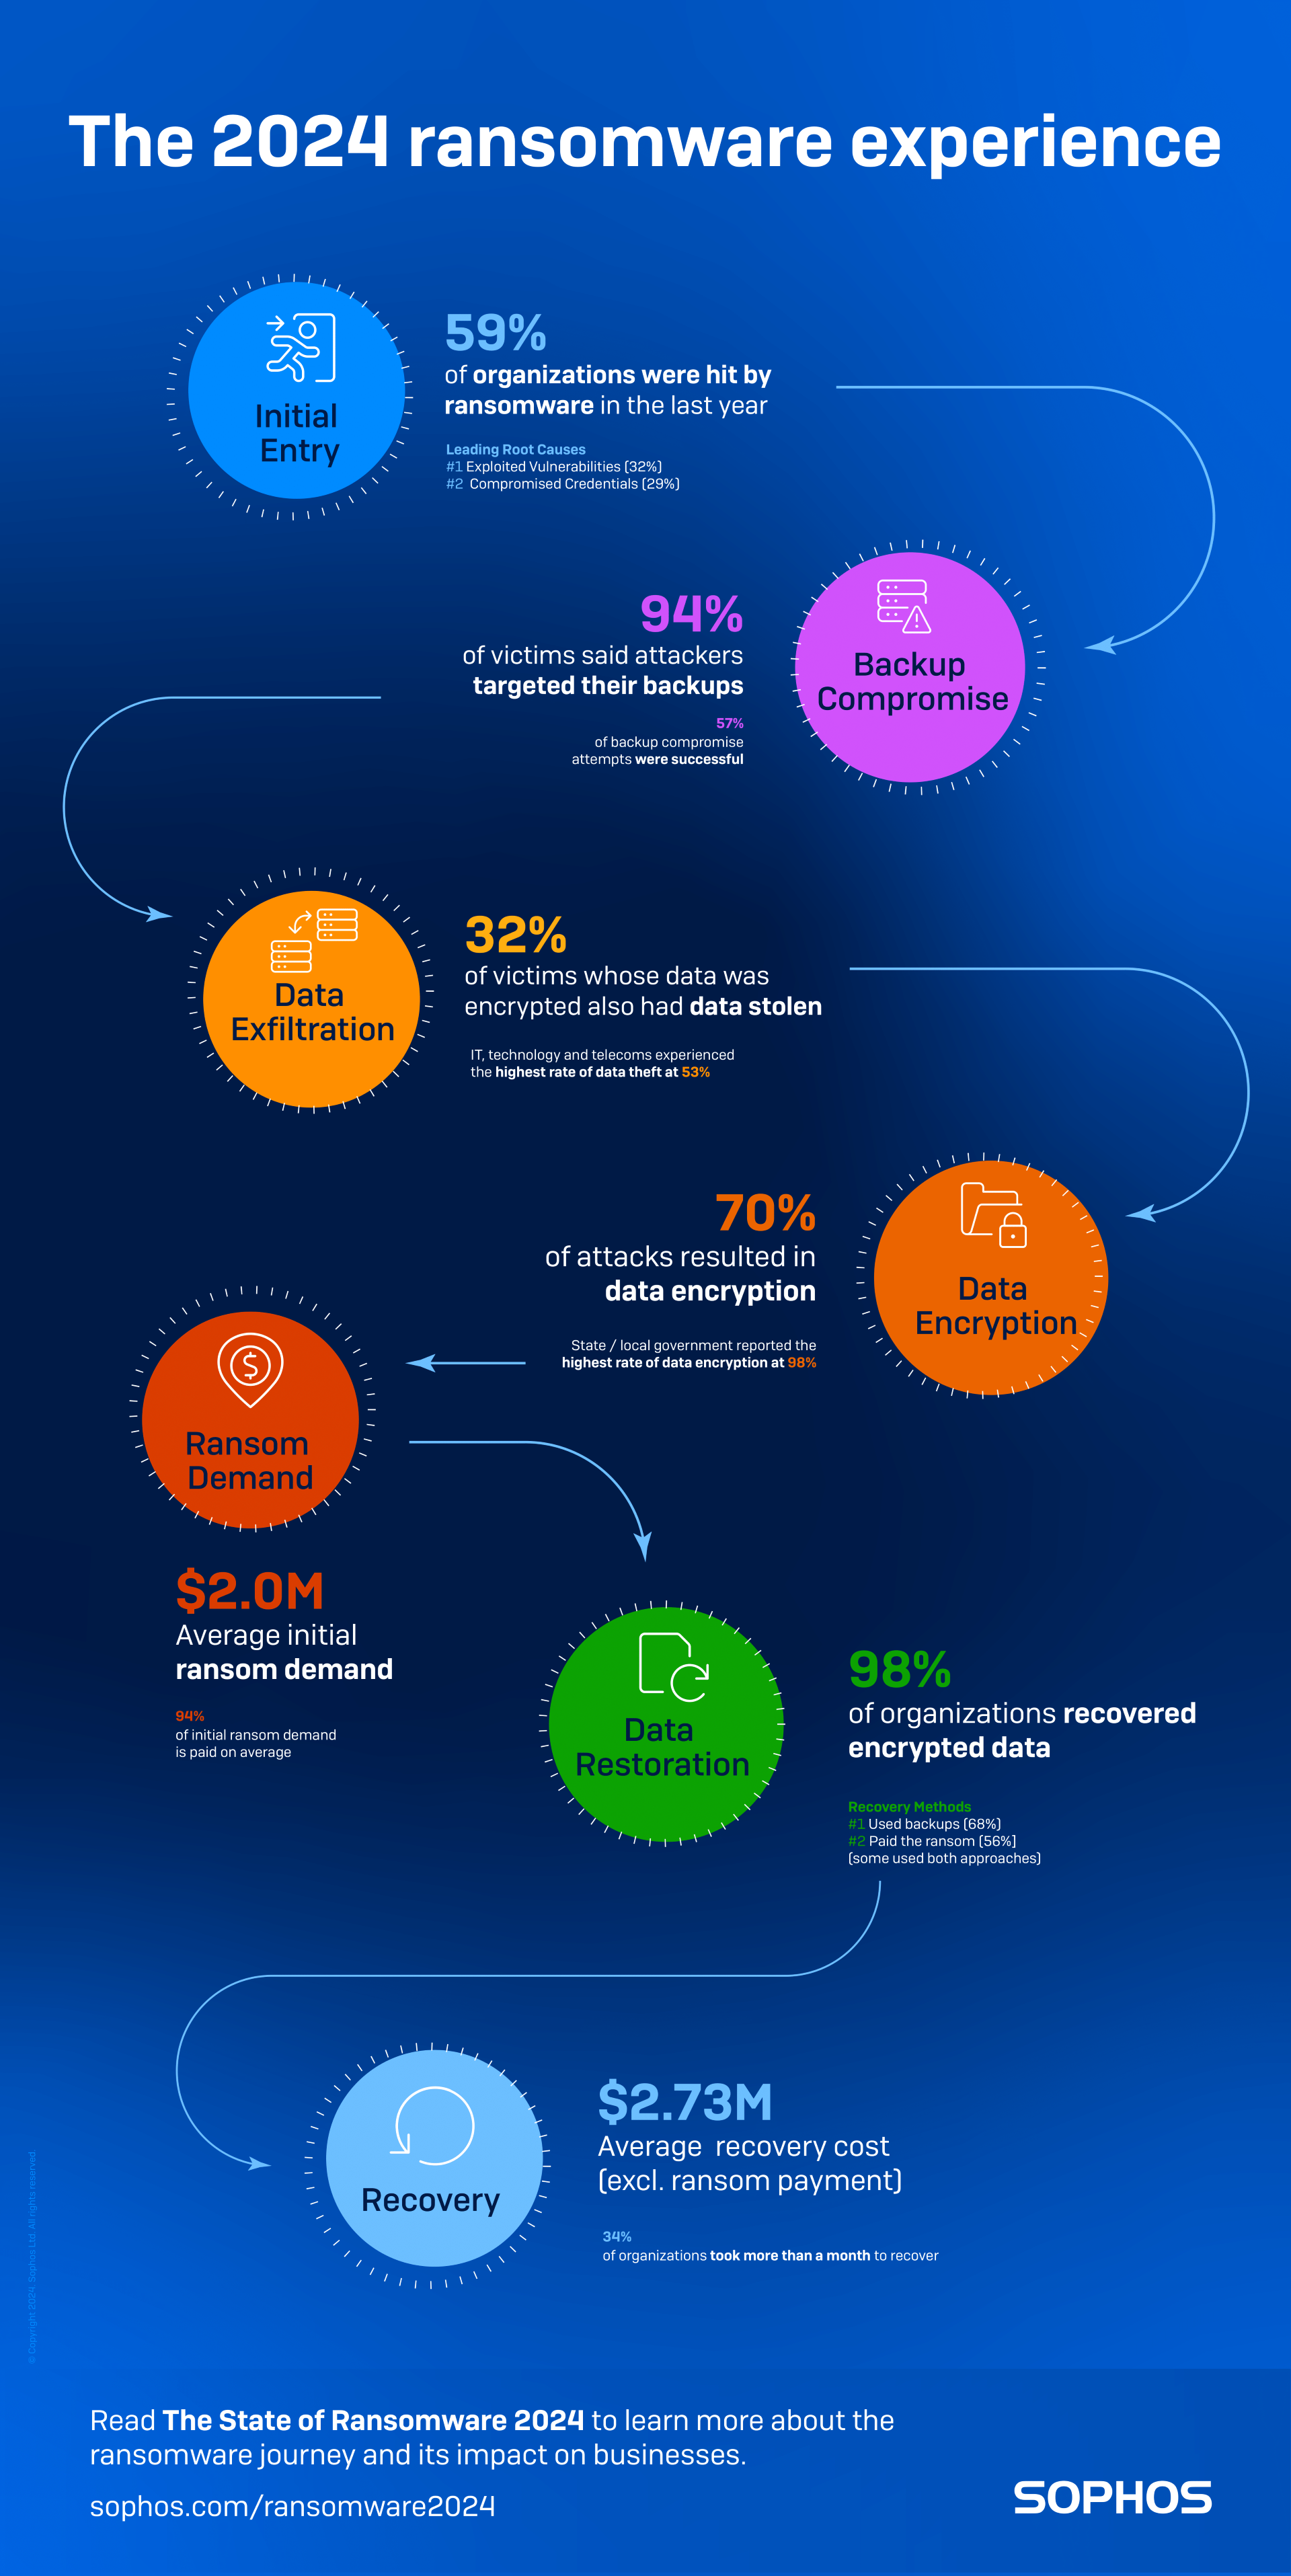
\includegraphics[width=0.5\textwidth]{Immagini/backup_and_d_r_statistics_2.png}
                \caption{Report di Sophos sui ransomware nel 2024 \cite{sophos_rep_b_d_r_ransomware}.}
                \label{fig:ransomware_rep}
            \end{figure}
        
        Esistono inoltre diverse tipologie di backup, e la scelta del sistema da usare dipende dalle esigenze specifiche dell'organizzazione e dai vincoli di budget, con opzioni che includono backup completi, incrementali, differenziali e la protezione continua dei dati, CDP, ognuna con vantaggi e limitazioni specifiche.\\ 
        I backup completi catturano tutti i dati regolarmente, offrendo una protezione esaustiva e semplificando il processo di ripristino, poiché richiedono solo l'ultimo backup per recuperare i dati. Tuttavia, questo approccio richiede spazio di archiviazione significativo e tempi di esecuzione prolungati, rendendolo meno pratico per ambienti con grandi volumi di dati o risorse limitate.

        I backup incrementali, invece, si concentrano solo sulle modifiche apportate ai dati dall'ultimo backup, offrendo efficienza in termini di spazio e tempo. Questo metodo riduce il carico sulle risorse di archiviazione e accelera il processo di backup, ma necessita di un backup completo per il ripristino totale, aumentando la complessità e il tempo richiesto in caso di recupero.
        
        I backup differenziali rappresentano un compromesso tra efficienza e velocità di recupero, poiché salvano tutte le modifiche apportate dal precedente backup completo. Rispetto ai backup incrementali, semplificano il processo di ripristino, ma richiedono più spazio di archiviazione man mano che il tempo tra due backup completi aumenta.
        
        Il CDP consente la replica in tempo reale, riducendo al minimo la perdita di dati anche durante frequenti interruzioni. Questo approccio è particolarmente utile per organizzazioni che non possono tollerare alcuna perdita di dati, ma richiede infrastrutture robuste e può comportare costi elevati, sia in termini di hardware che di larghezza di banda.
        I sistemi di backup efficaci si basano su componenti chiave come software di backup automatizzato, soluzioni di archiviazione locale, cloud o nastri, e infrastrutture di rete progettate per garantire trasferimenti sicuri ed efficienti. Le strategie di implementazione variano tra backup locale, remoto e cloud, con la regola 3-2-1 che offre un approccio bilanciato per la protezione dei dati. Per massimizzare l'efficacia, è fondamentale adottare best practice come test regolari, politiche chiare per la gestione dei dati, misure di sicurezza robuste e automazione dei processi. Tuttavia, l'implementazione del backup di rete presenta sfide significative, tra cui la complessità della gestione in reti distribuite, i costi elevati, la necessità di scalabilità e la crescente minaccia di attacchi informatici. Un'implementazione di successo richiede una pianificazione accurata, valutando dati critici, tempi di inattività accettabili e vincoli di budget, seguita da una configurazione attenta, test approfonditi e formazione degli utenti, con un monitoraggio continuo per garantire il corretto funzionamento e l'adattamento alle esigenze future.
        
    \subsection{Formazione e Coordinazione dei Reparti IT}
        L’introduzione di nuovi strumenti IT in azienda richiede una formazione adeguata per garantire che i dipendenti siano in grado di utilizzarli efficacemente, minimizzando interruzioni e massimizzando la produttività. Una formazione insufficiente può portare a errori operativi, violazioni della sicurezza e un uso limitato delle funzionalità, come dimostra il caso Target del 2013, in cui la mancanza di preparazione ha causato una grave violazione dei dati \cite{target_2013_breach}.

        Prima di avviare la formazione, è fondamentale valutare il livello di competenza attuale dei dipendenti, identificare gli obiettivi formativi e selezionare gli strumenti IT più adatti alle esigenze aziendali. La pianificazione deve includere tempistiche realistiche, risorse necessarie e tappe di monitoraggio per garantire un approccio strutturato.
        
        I metodi di formazione devono essere diversificati per adattarsi ai diversi stili di apprendimento. I workshop favoriscono l'apprendimento collaborativo, l'e-learning offre flessibilità per i dipendenti remoti, mentre le sessioni pratiche permettono di acquisire esperienza diretta. La scelta tra formatori interni ed esterni dipende dalla complessità dello strumento e dalle esigenze organizzative, con una combinazione spesso ideale per coprire sia aspetti tecnici che organizzativi. Materiali come manuali, video tutorial e guide rapide sono essenziali per supportare l'apprendimento.
        
        Per mantenere l'impegno dei dipendenti, è importante evidenziare i benefici degli strumenti per il loro ruolo, integrando elementi interattivi come quiz o esercitazioni pratiche. Incentivi e un ambiente favorevole alle domande possono ulteriormente motivare il personale.
        
        L’implementazione del programma di formazione deve seguire un approccio graduale, iniziando con piccoli gruppi per raccogliere feedback e affinare il processo. Le sessioni vanno programmate in orari non critici, garantendo l’accesso a tutte le risorse necessarie, come software aggiornati e ambienti di prova realistici. Durante la formazione, è cruciale monitorare i progressi e raccogliere feedback per apportare miglioramenti in tempo reale.
        
        Dopo la formazione, un supporto continuo è essenziale per risolvere dubbi e prevenire problemi. Promuovere una cultura di apprendimento continuo e offrire corsi di aggiornamento periodici aiuta i dipendenti a rimanere al passo con le evoluzioni degli strumenti. Monitoraggi regolari e valutazioni delle prestazioni consentono di misurare l’efficacia del programma e identificare aree di miglioramento.
        
        Casi di studio evidenziano l’importanza di una formazione ben strutturata: un’azienda di vendita al dettaglio ha aumentato l’efficienza operativa del 25\% grazie a un approccio misto di workshop, e-learning e sessioni pratiche, mentre una società finanziaria ha fallito nell’adozione di un nuovo software a causa di una formazione inadeguata.
        
        Le principali sfide nella formazione IT includono la resistenza al cambiamento, risorse limitate e la diversità nei ritmi di apprendimento. Soluzioni come l'e-learning, il coinvolgimento precoce dei dipendenti e l’offerta di metodi formativi vari possono mitigare questi ostacoli. Infine, la valutazione del successo della formazione si basa su metriche come aumento della produttività, riduzione degli errori e feedback qualitativo, che guidano eventuali aggiustamenti futuri.


\section{Penetration Testing - VAPT}
    Individuare le vulnerabilità nei sistemi accessibili sia internamente che esternamente è fondamentale per valutare il livello di rischio di un'organizzazione. Effettuare regolarmente controlli delle vulnerabilità, tramite scansioni automatizzate e revisioni manuali, permette di stabilire le priorità per le attività di mitigazione e di aggiornare le politiche di sicurezza. Adottare questo approccio preventivo è essenziale per difendersi da possibili attacchi e garantire il rispetto delle normative in materia di sicurezza informatica. Dato poi l'esponenziale evoluzione della tecnologia, anche gli attacchi sono diventati sempre più complessi. Uno dei metodi migliori per capire le vulnerabilità della propria rete è quello del \textbf{Vulnerability Assessment and Penetration Testing, VAPT}.\\
    Questa tecnica aiuta le organizzazioni a capire se la propria infrastruttura informatica funziona a dovere. Notiamo che questa strategia è composta da due fasi, la prima \textbf{VA}, per scovare le vulnerabilità e la seconda, \textbf{PT}, dove si provano a sfruttare queste vulnerabilità per ottenere accessi non autorizzati ed effettuare possibili attività dannose. Questo programma ci restituisce molte informazioni utili su quali possono essere i pericoli della nostra azienda e sull'entità dei danni che possono essere inflitti da un potenziale attacco.

    \subsection{Le Vulnerabilità}
        In genere gli attaccanti provano a sfruttare falle già note sperando (e riuscendo molto spesso a trovarle) in aggiornamenti mancati, dovuti a scarse politiche di aggiornamento o alla novità della falla trovata. Per mettere in sicurezza la rete, trovare queste vulnerabilità è fondamentale. Molte organizzazioni e framework citati precedentemente richiedono una regolarità nei VA, per accertarsi di avere una rete sicura; questo è particolarmente vero per le PCI DSS\footnote{Fonte: Wikipedia (\url{https://it.wikipedia.org/wiki/Payment_Card_Industry_Data_Security_Standard})} \cite{scada_system}, \cite{VAPT_Techniques}.
        Analizzando i tipi di vulnerabilità, capiamo che uno dei grandi problemi che viene riscontrato è come queste siano categorizzate; infatti, per non confondersi, sono state create delle organizzazioni per gestire al meglio questo compito come la CVE e la CWE, entrambe collegate alla MITRE di cui abbiamo parlato in precedenza. La Common Vulnerabilities and Exposure List, \textbf{CVE} è uno schema standardizzato dove vengono nominate in base a una convenzione le vulnerabilità, rendendone più facile la documentazione~\cite{cve}. La Common Weakness Enumeration, \textbf{CWE}, è invece un sistema che provvede a categorizzare queste vulnerabilità~\cite{cwe}.
        Il processo di Vulnerability assessment si divide in 4 fasi che sono:
        \begin{itemize}
            \item \textbf{Target Discovery}. Vengono raccolte le informazioni essenziali sul sistema da analizzare, come dettagli su reti, tecnologie utilizzate, applicazioni e infrastrutture. Questi dati permettono di comprendere l'architettura di sicurezza del target e definire le strategie di test. Tra le attività svolte ci sono, ad esempio, lo scanning Whois per ottenere informazioni sul dominio e l'analisi degli header HTTP per valutare le risposte del server web. Qui è dove vengono concentrate la maggior parte delle risorse.
            \item \textbf{Scanning}.  Viene analizzato l'intero sistema per individuare vulnerabilità come servizi non necessari, porte aperte, connessioni remote o password deboli. Utilizzano strumenti e tecniche specifiche, come lo Half TCP Scan: inviano un pacchetto TCP\textunderscore SYN alla porta target e, in base alla risposta (ACK per porta aperta, RST per chiusa, timeout per non risposta), determinano lo stato delle porte. Questo metodo è efficiente perché evita il completamento del processo di handshake TCP, riducendo i tempi e abbassando le probabilità di far scattare un IDS o IPS. Questa tecnica è presente anche nello strumento nmap\footnote{Sito: Nmap (\url{https://nmap.org/})} di cui parleremo dopo. Successivamente, con strumenti automatizzati, eseguono scansioni di rete e applicazioni web per identificare errori di configurazione o criticità, generando report dettagliati sui rischi rilevati.
            \item \textbf{Result Analysis}. Valutiamo  le vulnerabilità e le minacce individuate durante lo scanning. L'obiettivo è selezionare e classificare i problemi in base alla loro gravità e all'impatto potenziale sul sistema. Poiché i dati iniziali spesso includono molti falsi positivi, questa fase serve a filtrarli, ottenendo una lista più precisa e affidabile. Le vulnerabilità vengono quindi ordinate per priorità, creando un elenco finale che viene comunicato al team per la risoluzione o per ulteriori approfondimenti.
            \item \textbf{Reporting}. Documentiamo tutte le operazioni e i risultati ottenuti durante la valutazione delle vulnerabilità, producendo un report dettagliato che elenca le vulnerabilità identificate, il loro livello di gravità e altre informazioni rilevanti. Questo documento serve all'organizzazione per pianificare interventi correttivi.
        \end{itemize}

        \begin{figure}[h!]
            \centering
                \begin{minipage}{0.5\textwidth}
                    \centering
                    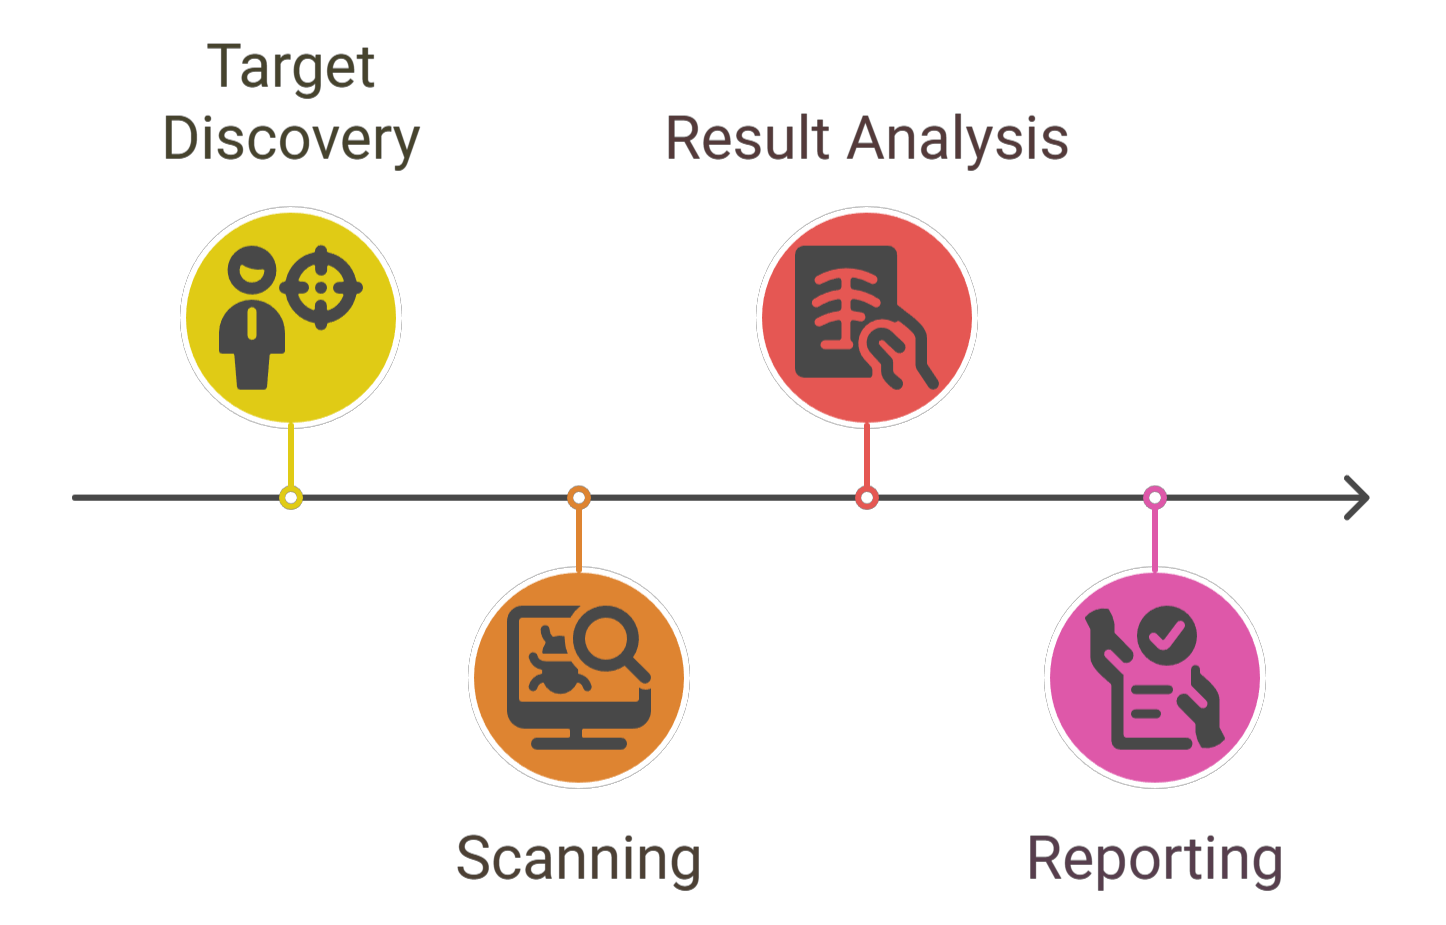
\includegraphics[width=1.0\textwidth]{Immagini/VA_phases_pentesting.png}
                    \caption{Le fasi nel Vulnerability Assessment.}
                \end{minipage}\hfill
                \begin{minipage}{0.5\textwidth}
                    \centering
                    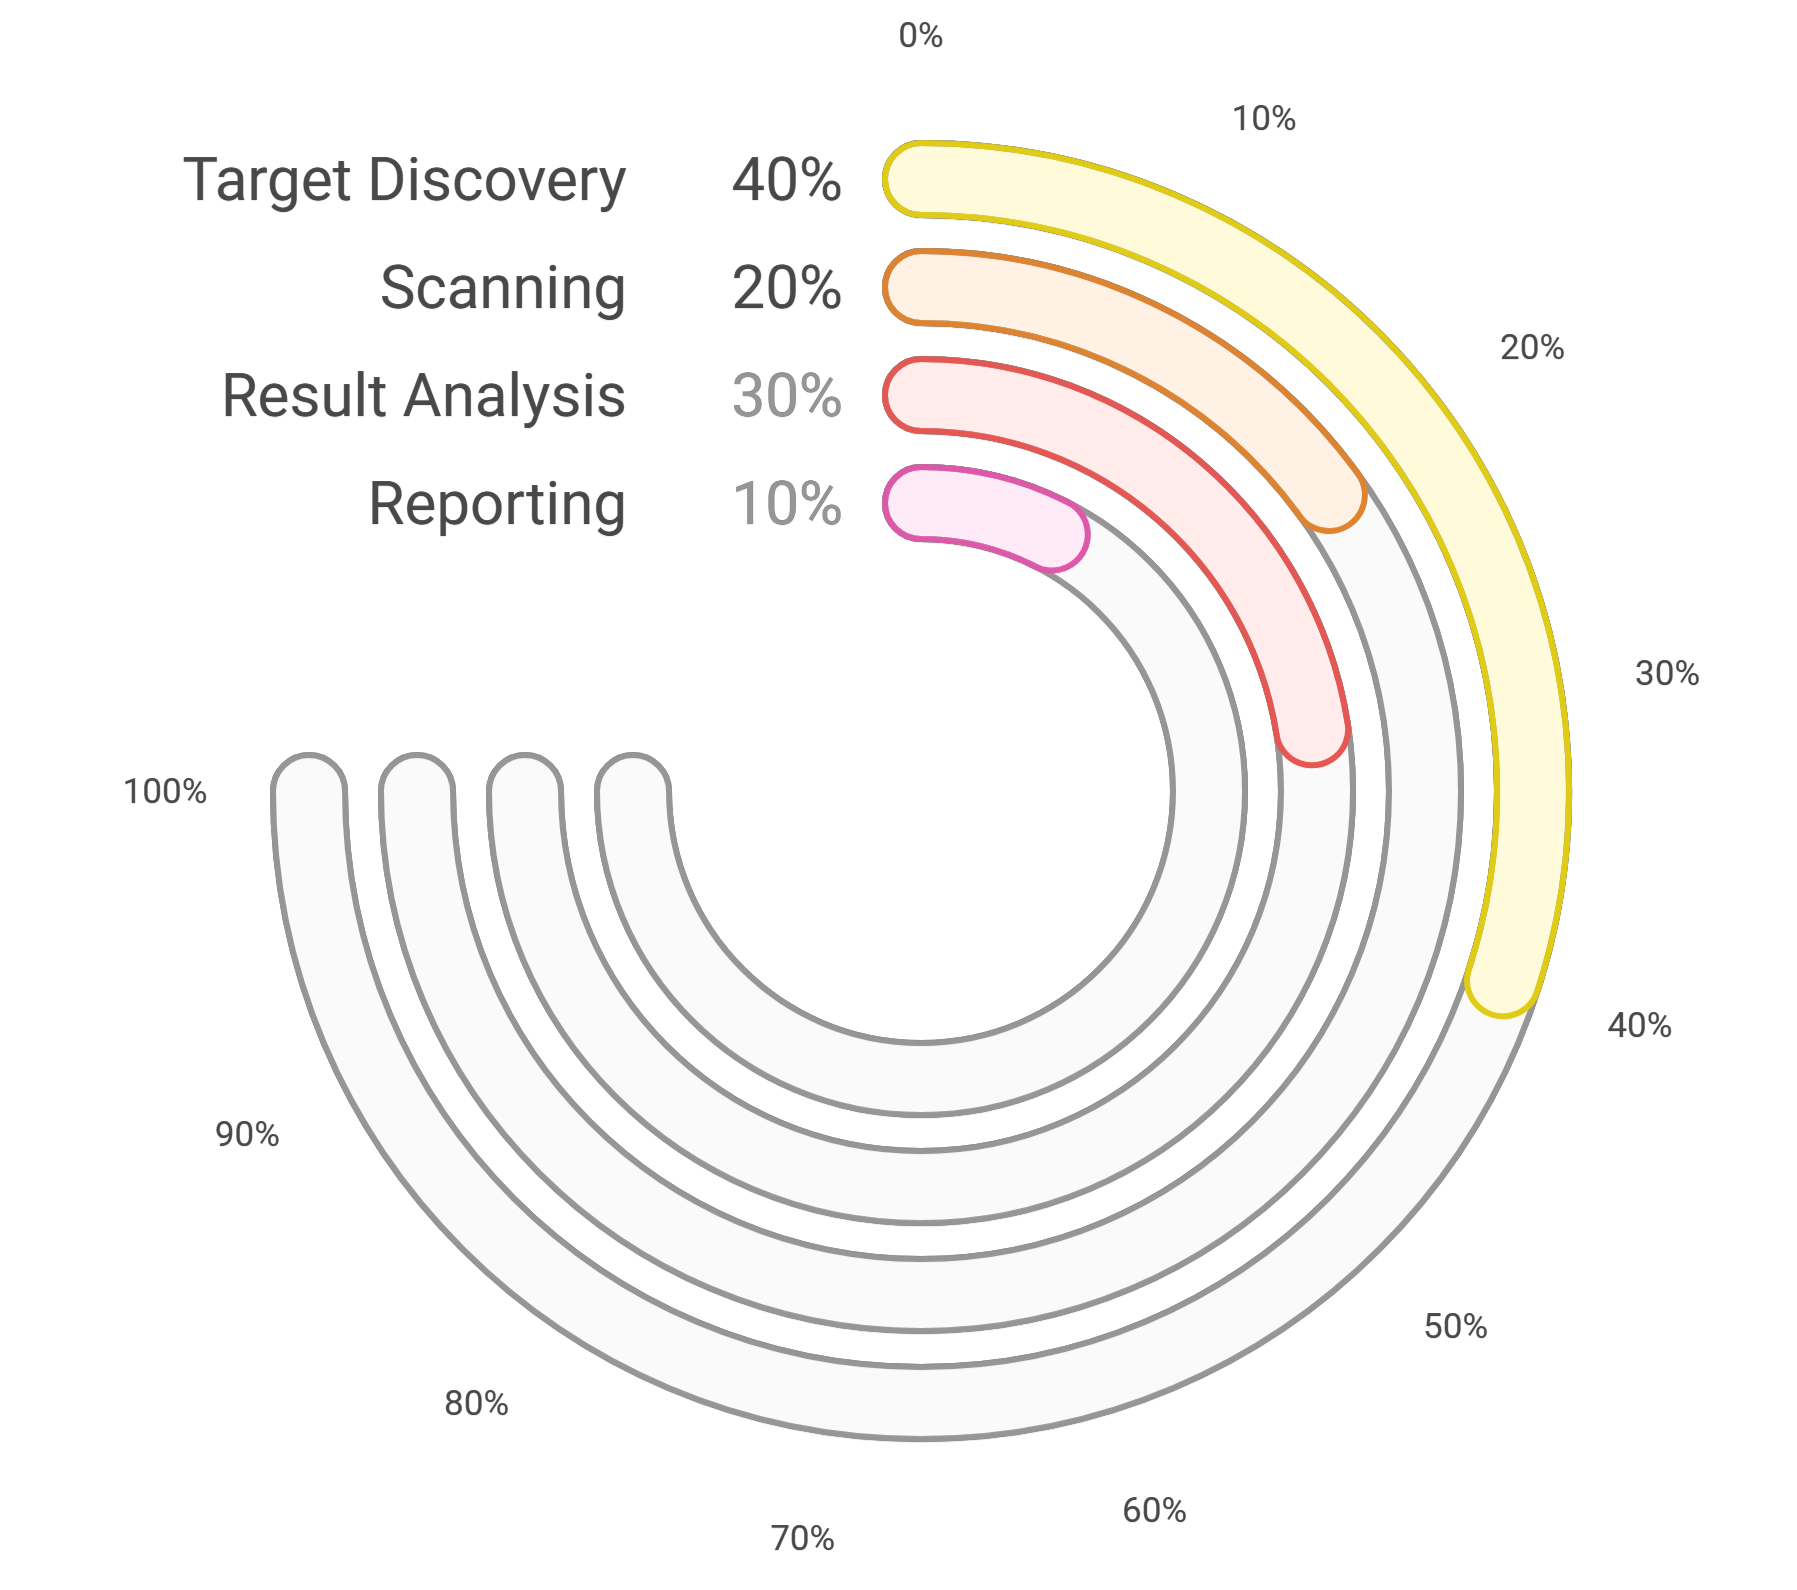
\includegraphics[width=1.0\textwidth]{Immagini/VA_workoload_percentage.png}
                    \caption{Percentuale del lavoro richiesto per le singole fasi \cite{VAPT_Techniques}.}
                \end{minipage}
        \end{figure}

        \subsubsection{Tecniche di Vulnerability Assessment}
            Questa strategia si può effettuare in due modi, manualmente o automaticamente.
            Nel \textbf{testing manuale}, il tester usa le sue competenze e sottopone l'obiettivo a vari test e osserva manualmente i risultati e i cambiamenti, i quali, se non sono in linea con quello che si aspetta, fanno dichiarare il software come vulnerabile. A sua volta, il metodo manuale viene diviso in:
            \begin{itemize}
                \item \textbf{Test Manuale Esplorativo}. Qua il tester naviga per il sistema trovando vulnerabilità senza un piano d'azione. L'affidabilità di questa tecnica è puramente basata su chi conduce il test \cite{vulnerability_assessment_techniques}.
                \item \textbf{Test Manuale Sistematico}. Questa tecnica abbiamo un piano d'azione definito, chiamato Test Plan. Qua il tester studia il sistema, i suoi componenti e le sue caratteristiche, sulle quali sviluppa un test plan efficiente e ad hoc per il sistema.
            \end{itemize}

            Invece nel \textbf{testing automatico}, il tester utilizza strumenti automatici per eseguire test ripetitivi, riducendo il tempo e l'intervento umano. Questi strumenti confrontano i risultati attesi con quelli reali del sistema, segnalando anomalie che potrebbero indicare vulnerabilità o errori di configurazione \cite{vulnerability_assessment_techniques}. Nel testing automatico vengono usate due tecniche:
            \begin{itemize}
                \item \textbf{Analisi statica}. Valuta il sistema e i suoi componenti basandosi sulla sua forma, struttura, contenuto o documentazione, che in ogni caso non richiede l'esecuzione del programma. A differenza della code review, che è manuale, questa tecnica si avvale di tool automatizzati, risultando più efficiente, soprattutto per il codice sorgente. Questa tecnica è ulteriormente caratterizzata in \textbf{Static Analysis for Source Code} e \textbf{Static Analysis for Machine Code}~\cite{static_analysis}.
                \item \textbf{Fuzzing}. Questa tecnica invia input casuali, invalidi o inaspettati al sistema per rilevare crash o comportamenti anomali. È efficace contro vulnerabilità come buffer overflow o SQL injection, ma meno utile contro minacce come keylogger. Si divide in due approcci:
                    \begin{itemize}
                        \item \textbf{Mutation Based Fuzzing}. Modifica gli input in modo casuale senza conoscere il formato, come ad esempio il bit-flipping.
                        \item \textbf{Generation Based Fuzzing}. Richiede una comprensione dettagliata del formato dei dati per generare input mirati.
                    \end{itemize}
            \end{itemize}

            Ogni tecnica ha vantaggi e limiti. Ad esempio, il fuzzing mutation-based è veloce ma poco preciso, mentre quello generation-based è più accurato ma complesso. La scelta della tecnica dipende dal tipo di target e dagli obiettivi del test: un tester esperto deve valutare pro e contro per ottimizzare i risultati ed evitare rischi inutili.

    \subsection{Penetration Testing}
        Il penetration testing è un processo che simula l'acquisizione illegittima di autorità legittima per valutare la sicurezza di un sistema. È uno strumento cruciale per le aziende, poiché permette di identificare rischi prima che si trasformino in violazioni concrete, proteggendo l'organizzazione da perdite finanziarie e danni alla reputazione~\cite{pen_testing}. Il processo si divide in quattro fasi principali e sono:
        \begin{itemize}
            \item \textbf{Planning and Preparation Phase}. Qua il tester e l'organizzazione concordano tempi, ambito e modalità del test. Viene raccolta informazioni sul target attraverso ricognizione passiva, senza interagire direttamente con la rete, e ricognizione attiva, con test diretti per ottenere risposte dal sistema.
            \item \textbf{Detection and Penetration Phase}. Il tester sfrutta strumenti e tecniche per compromettere il sistema, sfruttando vulnerabilità logiche o fisiche. Esempi includono l'acquisizione dell'accesso iniziale (perimeter penetration) e l'escalation dei privilegi.
            \item \textbf{Post Exploitation and Data Ex-filtration}. Qua documentiamo i percorsi per accedere ai dati sensibili, valutando punti di accesso, impostazioni di configurazione e impatto sui canali di comunicazione.
            \item \textbf{Reporting and Clean Up}. Viene in fine redatto un report dettagliato sulle vulnerabilità identificate, le modalità di sfruttamento e le raccomandazioni per mitigarle. Si eliminano inoltre tutti gli elementi creati durante il test.
        \end{itemize}

        \begin{figure}[h!]
            \centering
                \begin{minipage}{0.5\textwidth}
                    \centering
                    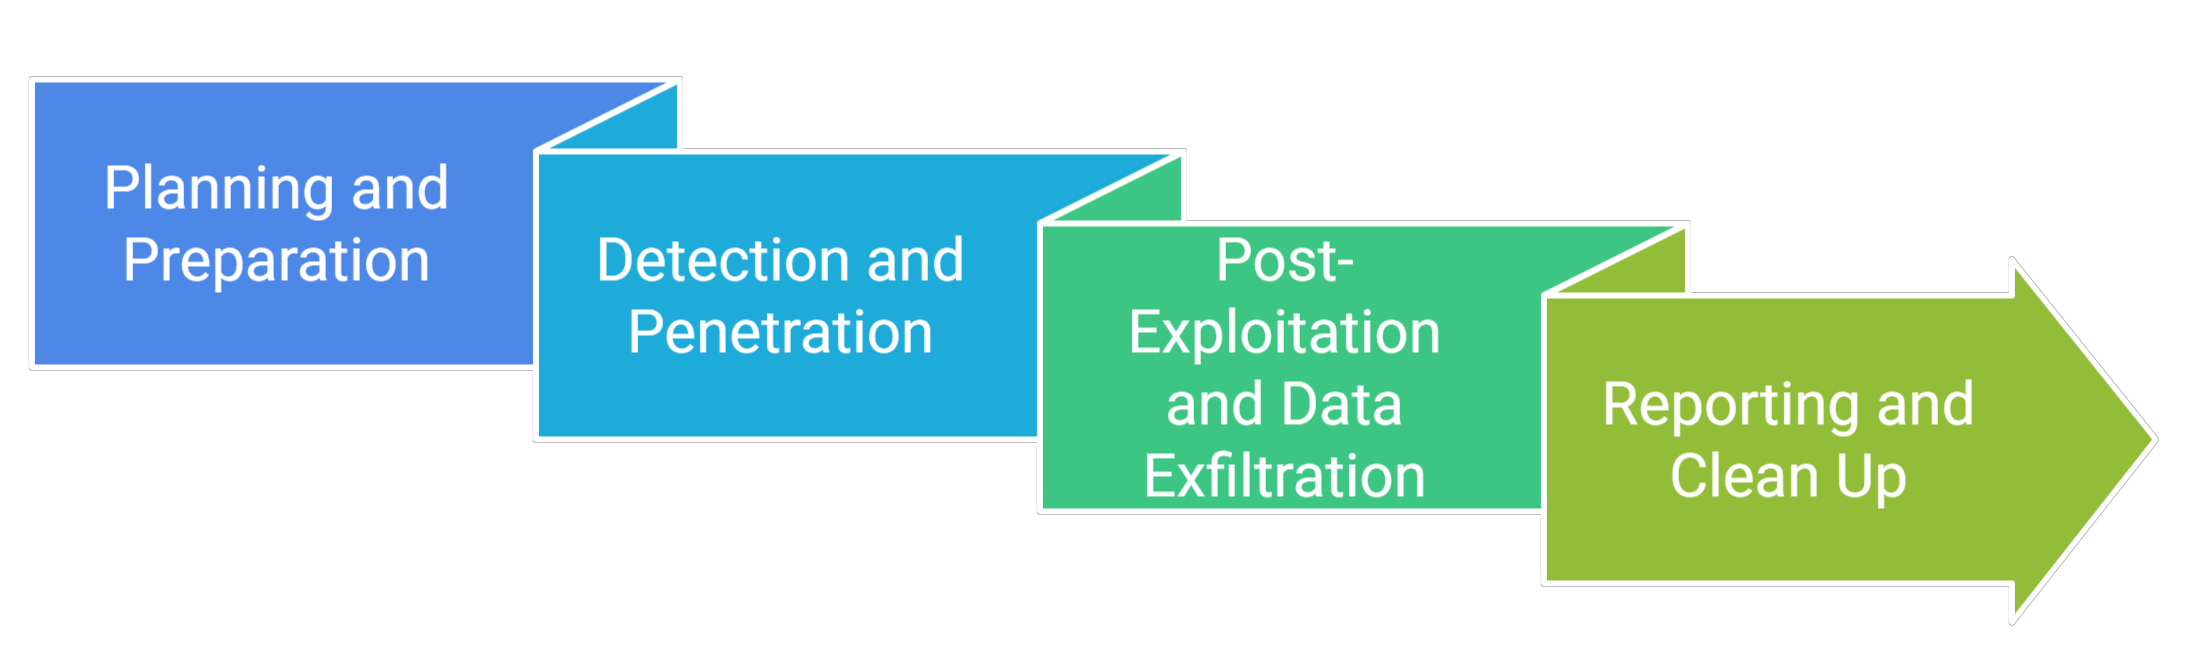
\includegraphics[width=1.0\textwidth]{Immagini/PT_phases_pentest_timeline.png}
                    \caption{Le fasi nel Pen Testing.}
                \end{minipage}\hfill
                \begin{minipage}{0.5\textwidth}
                    \centering
                    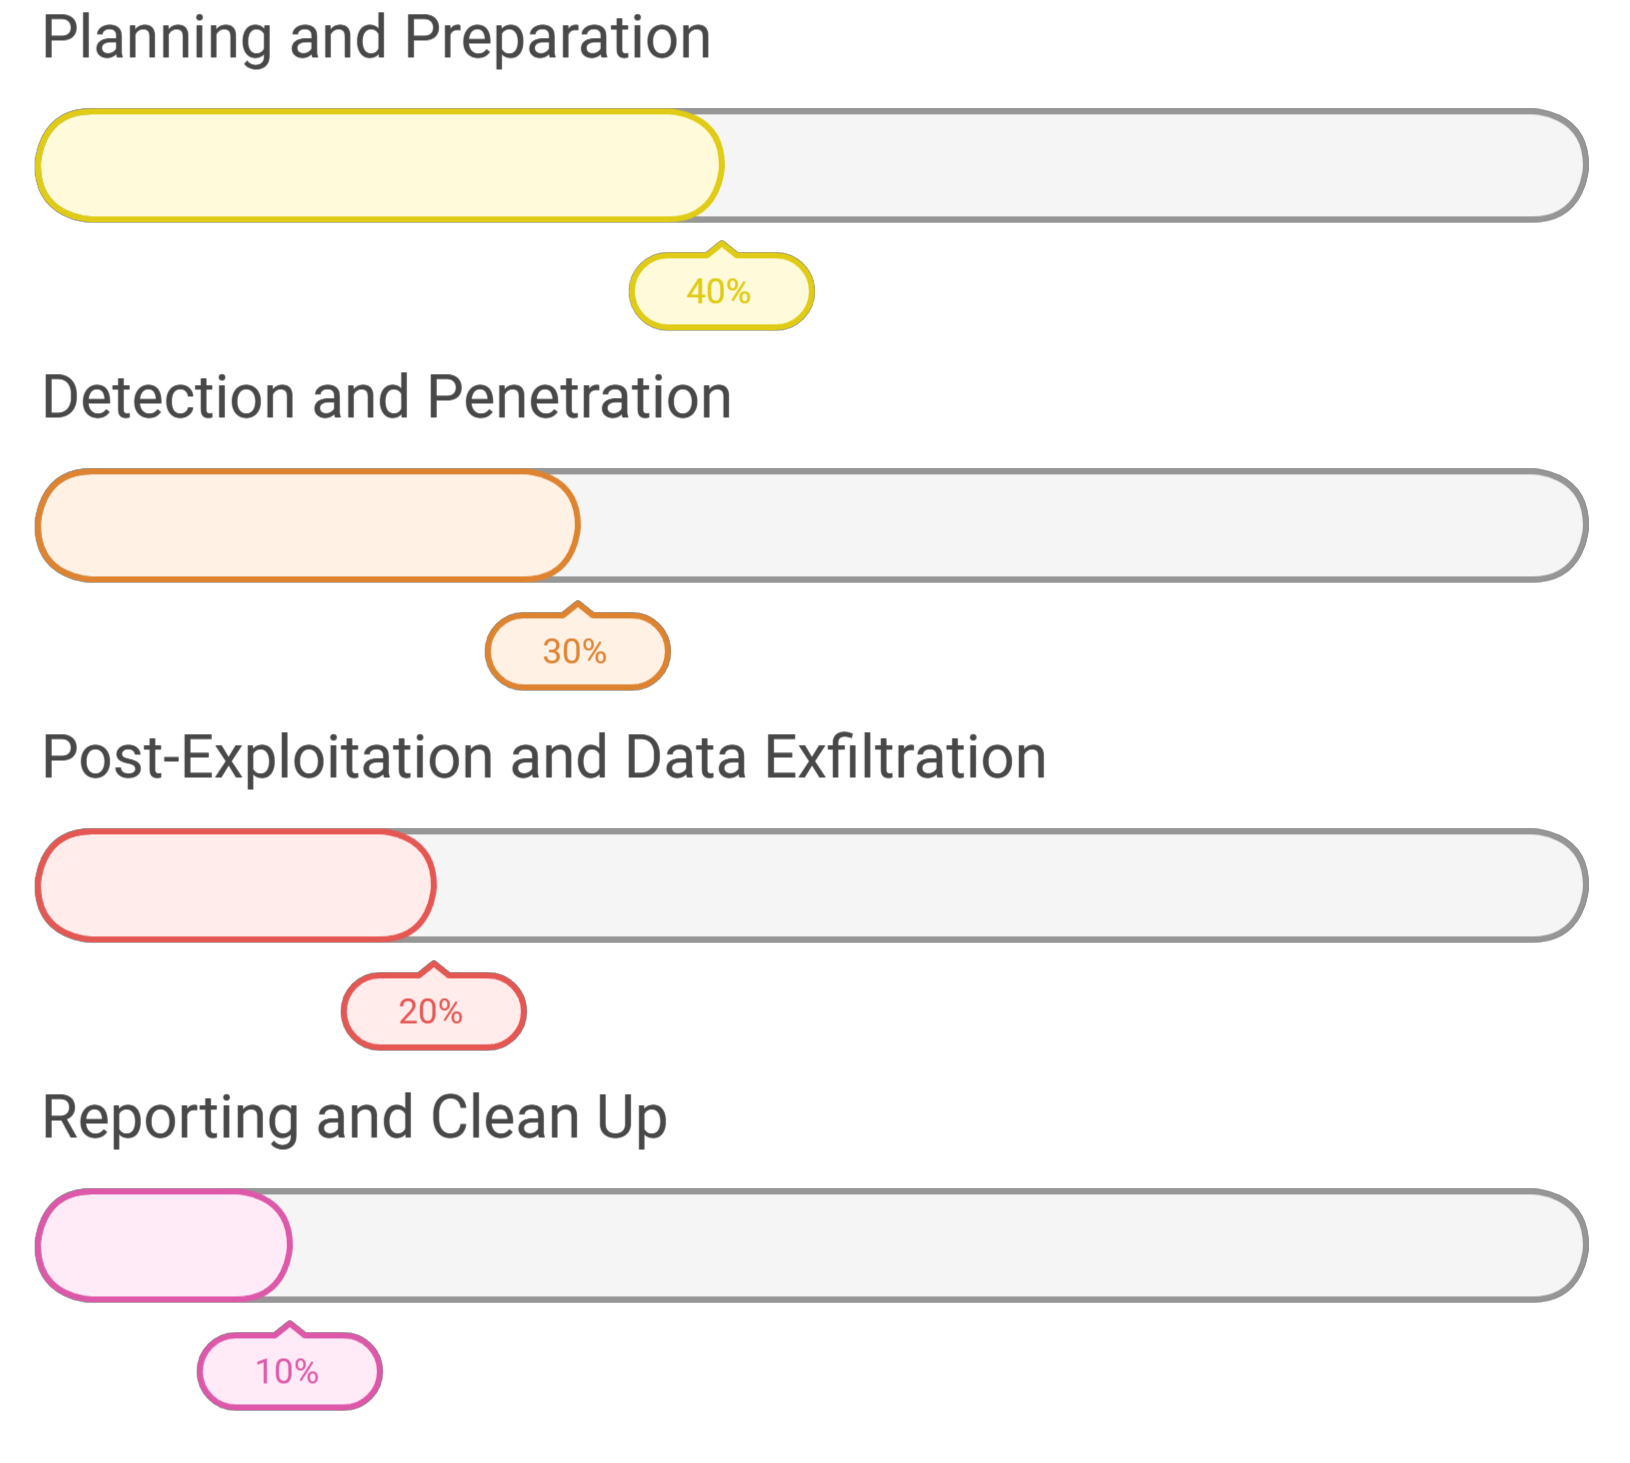
\includegraphics[width=1.0\textwidth]{Immagini/PT_workload_percentage_tablets.png}
                    \caption{Percentuale del lavoro richiesto per le singole fasi \cite{VAPT_Techniques}.}
                \end{minipage}
        \end{figure}

         \subsubsection{Strategie di Penetration Testing}
            Prima di analizzare queste strategie, notiamo come il MITRE ATT\&CK precedentemente citato sia molto usato nelle strategie di pentesting \cite{mitre_attt_ck_in_pentest}.
            Il penetration testing per siti web si basa su tre metodologie principali \cite{pen_testing}, ognuna con approcci e obiettivi distinti:
            \begin{itemize}
                \item \textbf{Black Box Testing}. Simula un attacco esterno, dove il tester non ha alcuna conoscenza preliminare del sito (codice, documentazione, configurazioni). Inizia con attività di ricognizione come scansione delle porte o mappatura della rete per identificare punti deboli, sfruttando poi strumenti automatizzati e tecniche manuali per violare il sistema. Questo approccio offre una visione realistica della sicurezza, poiché replica le condizioni di un aggressore reale, ma richiede tempo e risorse elevate a causa della necessità di raccogliere informazioni da zero\cite{black_box}.
                \item \textbf{White Box Testing}. In questo caso invece il tester ha accesso completo al codice sorgente, all'architettura e alla documentazione interna. Questo permette analisi approfondite, come scansioni avanzate o test sul design del sistema, identificando vulnerabilità prima del deployment. È ideale per ottimizzare la sicurezza in fase di sviluppo, ma potrebbe sovrastimare le difese, poiché un attaccante esterno non disporrebbe delle stesse informazioni. Inoltre, richiede competenze specializzate e può risultare costoso \cite{white_box}, \cite{white_box_2}.

\newpage
                
                \item \textbf{Grey Box Testing}. Qua combiniamo elementi delle prime due: il tester riceve informazioni parziali, come credenziali utente, diagrammi di rete, per simulare attacchi da parte di insider o hacker con accesso limitato. Ad esempio, potrebbe utilizzare dati forniti per eseguire attacchi brute-force o analizzare configurazioni specifiche. Offre un equilibrio tra realismo e profondità, ma dipende dalla collaborazione con gli amministratori e non riflette pienamente le minacce esterne pure \cite{grey_box}.
            \end{itemize}

            \begin{table}[!htbp]
                \begin{center}  
                    \begin{tabular}{|P{40mm}|P{25mm}|P{25mm}|P{35mm}|}  
                        \hline  
                        \multicolumn{4}{|c|}{\textbf{Confronto tra Black Box, White Box e Grey Box}} \\  
                        \hline  
                        \textbf{Aspetto di confronto} & \textbf{Black Box} & \textbf{White Box} & \textbf{Grey Box} \\  
                        \hline  
                        Informazioni sul target & Nessuna informazione o accesso & Accesso completo & Accesso parziale \\  
                        \hline  
                        Natura del testing & Test di accettazione utente & Solo sviluppatori/tester & Test di accettazione utente \\  
                        \hline  
                        Tempo e sforzo & Molto elevato & Ridotto & Intermedio \\  
                        \hline  
                        Granularità del test & Bassa & Alta & Media \\  
                        \hline  
                        Fondamenti & Eccezioni esterne (comportamenti interni sconosciuti) & Eccezioni interne/esterne (comportamenti noti) & Diagrammi di database e stati interni \\  
                        \hline  
                        Ambito del testing & Trial-and-error, limiti esterni & Dati e limiti interni & Limiti interni/esterni, overflow \\  
                        \hline  
                        Limitazioni & Non adatto per algoritmi & Adatto a tutti & Non adatto per algoritmi \\  
                        \hline  
                    \end{tabular}  
                    \caption{Confronto delle metodologie di testing \cite{VAPT_Techniques}.}  
                    \label{tab:confronto-testing}  
                \end{center}  
            \end{table}
        
        \newpage

        \subsubsection{Software per il VAPT}
        Vediamo ora due software, come Vuls e Nmap, entrambi open-source e utilizzati apposta per la scansione delle reti propedeutici al tracciamento delle vulnerabilità.
        \begin{figure}[H]
            \centering
            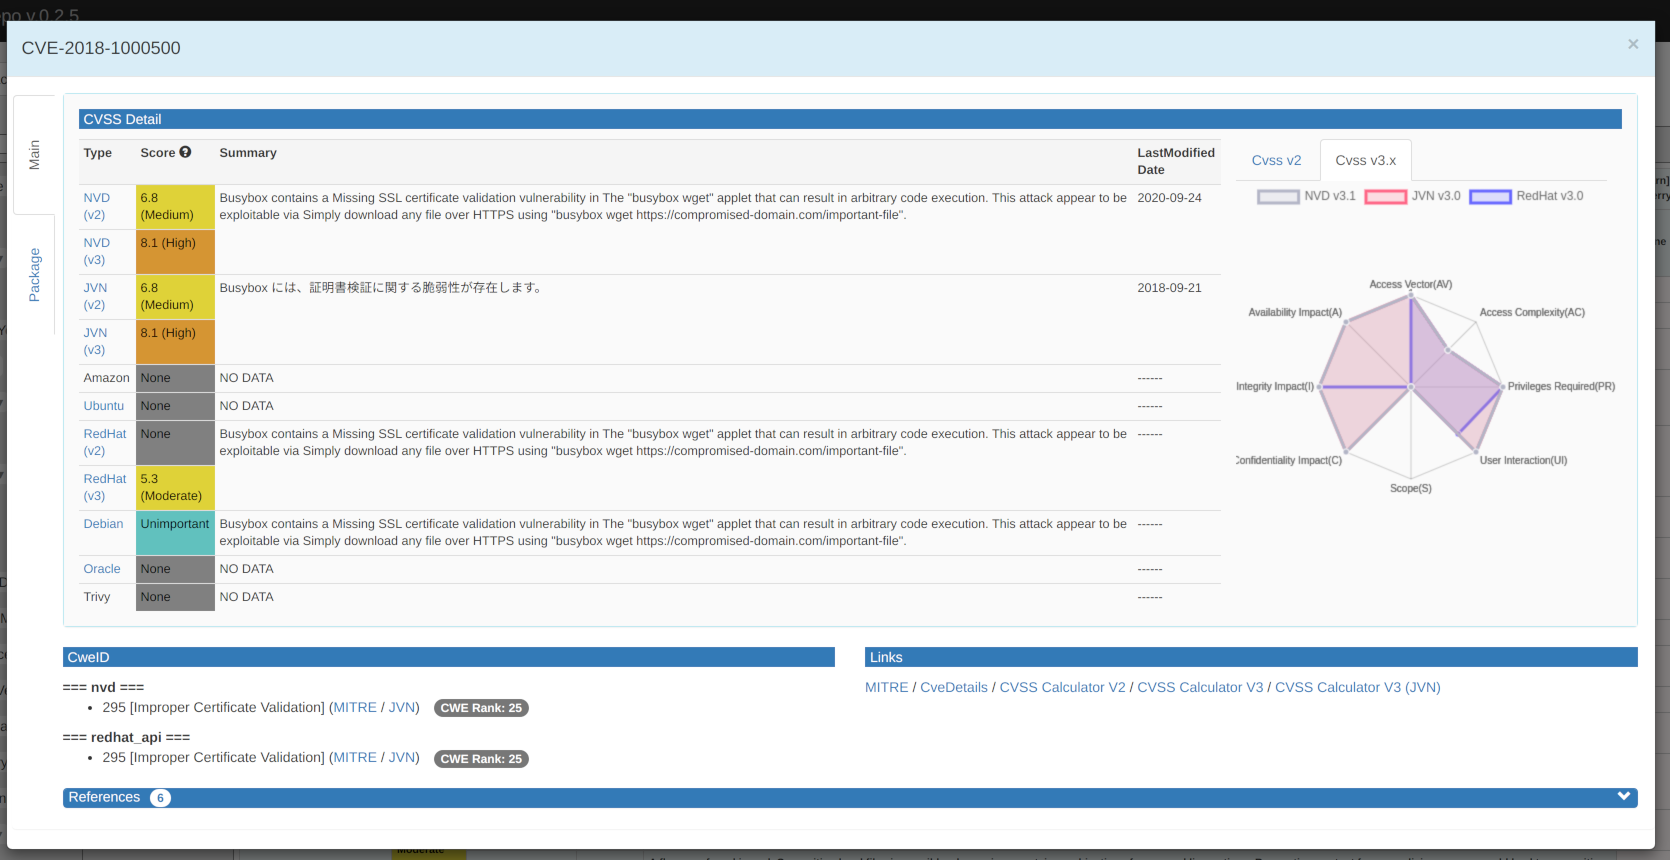
\includegraphics[width=1.0\textwidth]{Immagini/vuls_main_page.png}
            \caption{L'interfaccia web di Vuls\protect\footnotemark, con i dettagli di una vulnerabilità CVE, i punteggi di gravità CVSS e un grafico radar che riassume il livello di rischio, insieme a riferimenti e metadati utili per la gestione della minaccia.}
            \label{fig:vuls_main_page}
        \end{figure}
        \footnotetext{Fonte: Vuls (\url{https://vuls.io/docs/en/vulsrepo.html})}

        \footnotetext[15]{Fonte: Nmap (\url{https://nmap.org/})}
        \begin{figure}[H]
            \centering
            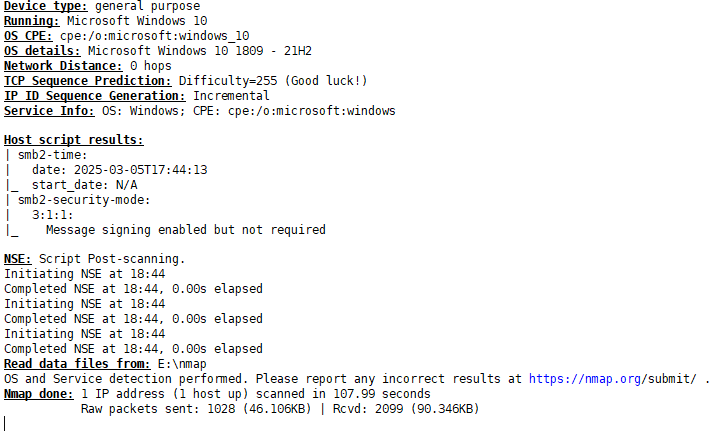
\includegraphics[width=1.0\textwidth]{Immagini/nmap_2.PNG}
            \caption{L'interfaccia gui di nmap\protect\footnotemark, rappresenta una scansione di una rete locale. Mostra i dettagli di un host trovato in rete.}
            \label{fig:nmap_scan_host}
        \end{figure}
        
        
        \begin{figure}[H]
            \centering
            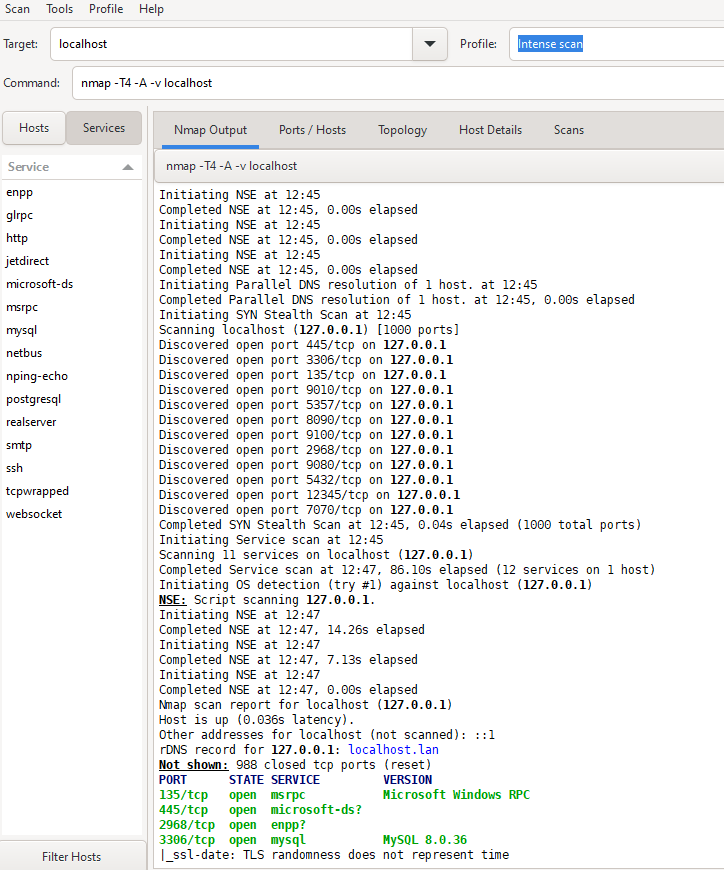
\includegraphics[width=1.0\textwidth]{Immagini/nmap.PNG}
            \caption{L'interfaccia gui di nmap, rappresenta una scansione di una rete locale. La scansione è stata effettuata in modalità “Intense Scan”\protect\footnotemark e l'output ci mostra le porte trovate aperte in quella rete e i servizi collegati a quella rete.}
            \label{fig:nmap_scan}
        \end{figure}
        \footnotetext{Fonte: Nmap (\url{https://nmap.org/book/zenmap-scanning.html})}